\documentclass[]{article}

% math packages
\usepackage{amsmath}
\usepackage{amsthm}
\usepackage{bm}

% for coloring in a table
%\usepackage[table,xcdraw]{xcolor}

% including graphics
\usepackage{graphicx}
\graphicspath{ {./images/} }

% drawing graphs
\usepackage{tikz-cd}
\usepackage{tikz}
\usetikzlibrary{shapes.geometric, arrows}
\tikzstyle{startstop} = [rectangle, rounded corners, minimum width=3cm, minimum height=1cm,text centered, draw=black, fill=red!10]
\tikzstyle{arrow} = [thick,->,>=stealth]

% hyperlinks
\usepackage{hyperref}

% some useful shortcuts
\DeclareMathOperator*{\argmax}{argmax}
\newcommand{\indep}{\perp\!\!\!\!\perp}
\newcommand{\blambda}{{\bm{\lambda}}}
\newcommand{\btheta}{{\bm{\theta}}}
\newcommand{\bpsi}{{\bm{\psi}}}

\newcommand{\by}{\mathbf{y}}

\usepackage{setspace}
\doublespacing

% Editing macros
\usepackage{color}
\newcommand\cmnt[2]{\qquad{{\color{red} \em #1---#2} \qquad}}
\newcommand\cmntM[1]{\cmnt{#1}{Miratrix}}
\newcommand\cmntC[1]{\cmnt{#1}{Che}}
\newcommand\awk{{{\color{red} {$\leftarrow$ Awkward phrasing}}\qquad}}
\newcommand\cmntMp[1]{{\color{red} $\leftarrow$ {\em #1 -Miratrix} \qquad}}



%opening
\title{Power calculations for detecting \\ individual site impacts}
\author{Jonathan Che \& Luke Miratrix}

\begin{document}

\maketitle

%\begin{abstract}
%\end{abstract}


\section{Introduction}

The usual question for multisite trials\textemdash randomized trials where each of a set of sites has individuals randomized into treatment and control\textemdash is whether the treatment worked \emph{on average overall}, even though the treatment may have different effects across sites.
When designing a multisite experiment there are power analysis tools designed to ensure a given design will achieve desired levels of power for this average effect.
There are even power formulas designed to ensure one can detect a given level of cross-site impact variation, if that is a quantity of interest.

But what if we are interested in the individual sites?
Typically, in a multisite experiment no individual site will be large enough to be well-powered, on its own, for detecting whether treatment at that site was actually effective.
This is, after all, why we frequently turn to multisite experiments: we seek to increase our overall power by averaging across a collection of underpowered, local, investigations.
That being said, the stakeholders at these local investigations will frequently want to know not whether the experiment worked overall, but whether it worked for them.
As researchers, we might also want to identify which sites are most likely to be the drivers of an overall effect.

We can get an approximate answer to these questions about individual sites by using multilevel or hierarchical Bayesian models to partially pool the individual site effects.
For each site, these models ``borrow strength'' from the other sites under the assumption that the sites are related.
This process results in point estimates for each of the individual sites that are shrunken towards the overall average estimated effect.

The construction of confidence intervals around these shrunken estimates requires some nuance.
There is an extensive literature concerning the construction of appropriate credible intervals for individual site effects under shrinkage (see Casella and Hwang (2012) for a thorough review; see He (1992), Hwang et al. (2009), and Armstrong et al. (2021) for relevant examples of these methods).
These credible intervals do not satisfy the frequentist definition of $\alpha$-level converage for the $\tau_j$ values; instead, they satisfy so-called Empirical Bayes (EB) coverage, which integrates the coverage probability over both the data and the parameters (Morris 1983).\footnote{Recall that frequentist coverage is defined as the probability that a random interval contains a fixed parameter $\theta$, where randomness is integrated over the distribution of the observed data.
EB coverage additionally integrates out the parameter $\theta$ over its prior distribution.}
This means that they only provide guarantees for \textit{average} coverage across sites, and not for coverage for any particular site.
These guarantees may not be sufficient for stakeholders in multisite trials specifically interested in knowing whether the experiment worked for their site.
For example, the inherent bias in shrunken point estimates raises concerns that only examining average coverage could mask systematic undercoverage for sites with extreme effects, which would be a problem for stakeholders at such sites.
Overall, the question of inference for particular site effects in multilevel models appears to remain fairly open (Armstrong et al. 2021), with limited guidance about best practices.

In this study, we focus on frequentist-style conditional power analyses for detecting a hypothesized effect for a specific site in a particular study design.
We consider finite-sample power/coverage conditional on given $\tau_j$ values instead of average power/coverage across the collection of $\tau_j$ values in a multisite trial.
Similar power analyses have previously been conducted for the overall average treatment effect and cross-site variation in multisite trials (e.g., Raudenbush \& Liu 2000, many others), but not for individual site-effect estimates.
Like these previous power analyses, our power analyses will require specification of the characteristics of the full multisite trial (e.g., its overall average treatment effect and cross-site variation), since the effect estimate for each site will generally depend on the full context.
The focus, however, will be on the power to detect individual site effects of a given size.

In this document, we first review how one might use multilevel and Bayesian models to report individual site-effect estimates.
We then propose simulation-based tools to estimate the power to detect an individual site effect of a given size in a multisite trial with given characteristics.
Finally, we conduct a simulation study to examine power for site-level treatment effects in multisite trials.
At this point, we also examine how poorly these site-level estimates perform in practice, and provide guidance on the overall business of individual site-effect estimation in the context of multisite trials.


\section{Detecting individual site effects}

In this section, we briefly review how to estimate individual site-level treatment effects in a multisite trial.
To make things concrete, assume a simple Normal multilevel model for individuals $i$ in sites $j$ of: 
\begin{align*}
	Y_{ij} &= \alpha_j + \tau_j Z_{ij} + \epsilon_{ij} \\
	\alpha_j &= \alpha + u_{0j} \\
	\tau_j &= \tau + u_{1j} \\
	\begin{pmatrix}
		u_{0j} \\ u_{1j}
	\end{pmatrix} &\sim N\left(
	\begin{pmatrix}
		0 \\ 0
	\end{pmatrix}, 
	\begin{bmatrix}
		\sigma^2_\alpha & \rho_{01} \\  & \sigma^2_\tau
	\end{bmatrix}\right) \\
	\epsilon_{ij} &\sim N(0, \sigma^2_y) ,
\end{align*}
for individual outcomes $Y_{ij}$, individual treatment indicators $Z_{ij}$, random site intercepts $\alpha_j$, and random site treatment effects $\tau_j$.
To simplify things, we will operate in effect-size units, assuming data are rescaled such that $Var(Y_{ij} \mid Z_{ij}=0) = 1$, i.e., that $\sigma^2_y + \sigma^2_\alpha = 1$.
This also implies that $ICC = \sigma^2_\alpha / (\sigma^2_y + \sigma^2_\alpha) = \sigma^2_\alpha$.
Finally, we set $\rho_{10} = 0$ so that intercept and treatment random effects are uncorrelated.

The simplest, completely unpooled test of whether there is a positive treatment effect within each site $j$ would be to drop the rest of the data and test the difference in means of the treatment and control groups within site $j$.
The power to detect effects locally in this manner is purely a function of the site sample size, variation in outcomes within the site, and the size of the true site average impact.
The typical formula for the standard error for site $j$'s impact estimate would then be:
$$ SE_j = \left[ \frac{1}{n_j} \frac{1}{(1-p_j)p_j} (1-ICC) \right]^{1/2} , $$ 
where $p_j$ is the proportion treated at site $j$.
For testing, we would estimate $\hat{\tau}_j$ and $\widehat{SE}_j$, the latter with a plug-in estimate of $\hat{\sigma}_j$ for site $j$.
We could either estimate $\hat{\sigma}_j$ with an interacted linear regression where we completely pool our residual variation across sites, or simply estimate the within-group variation at site $j$.
We would finally obtain $p$-values using $t = \hat{\tau}_j / \widehat{SE}_j$, referenced to a $t$ distribution with many degrees of freedom, assuming the site is not tiny.

A multisite analysis pools data across sites to try to improve effect estimates.
With a multilevel model, we first estimate the overall parameters, including the degree of cross site variation $\sigma^2_\tau$, and none of the individual site average impacts.
We then, in a second step, effectively shrink all the raw $\hat{\tau}_j$ towards the overall estimate of $\hat{\tau}$ to get $\tilde{\tau}_j$, shrinking more the lower our estimate of $\sigma^2_\tau$ is.
These $\tilde{\tau}_j$ are the Empirical Bayes estimates for the individual site impacts; while biased, they are known to be better point estimates (in terms of mean-squared error) for the full collection of true site-level impacts than the raw estimates $\hat{\tau}_j$.

Under a parametric or empirical Bayes framework, we can also obtain standard error estimates $\tilde{SE}_j$ for our $\tilde{\tau}_j$.
Using the estimate $\tilde{\tau}_j$ and standard error $\tilde{SE}_j$, we can finally conduct hypothesis testing as before, taking the test statistic of $t = \tilde{\tau}_j / \tilde{SE}_j$ as standard normal statistic and calculating a $p$-value as usual.
As discussed in the introduction, however, confidence intervals constructed using these standard errors do not satisfy frequentist coverage criteria, where, e.g., for a fixed $\tau_j$ the interval $(\tilde{\tau}_j \pm 1.96 \tilde{SE}_j)$ would cover $\tau_j$ 95\% of the time over repeated samples of the data.
Instead, they satisfy EB coverage, where appropriate coverage holds over repeated samples of the data \textit{and} $\tau_j$ from the data-generating Normal model.
In other words, hypothesis tests run in this way will not have the usual guarantees on Type-I error rate control for the site-specific effects.
That being said, they may perform decently well in practice.

Without shrinkage, power is simply a function of the un-shrunk standard error $SE_j$ and the true average effect $\tau_j$ for site $j$.
Given the shrinkage, the power to detect an individual site effect will additionally depend on the general size and distribution of average effects at other sites.
Of course, the most relevant parameter will be the individual site's average effect, but the distribution of impacts estimated at the other sites will affect how each site estimate is shrunk towards the overall average impact.
The question is how much this shrinkage helps or hurts the power and validity of the testing procedure, especially for those sites that actually have impacts far from the overall average.


\section{A simulation-based power calculator}

To calculate the power to detect an effect of a given size at an individual site in a multisite trial, we need to specify parameters for both the individual site of interest and its context.
While a typical power analysis for a single site only requires specification of a single hypothesized effect size (along with significance and power requirements), in a multisite trial the site's context, i.e., the number, size, and distribution of the other sites, will also affect the effect estimate for that site.
The question is then: for a given site of interest, \textit{within a given context of interest}, what is the chance of rejecting the null of no effect for that site?

We answer this question via simulation.
We simulate data using the model shown in the previous section.
To conduct our power analyses, we want to repeatedly generate our target site and an associated context, analyze the synthetic data, and record whether we have detected an effect.
The frequency with which we reject the null across our simulations is then the power for that site and context.
If the true site impact is 0, this power is the validity of the given hypothesis test, and we hope that it is near the specified confidence level $\alpha$ for the test.
The question of how exactly to specify our site of interest and its context, however, deserves some additional thought.
Below, we propose two general definitions for simulating a ``site of interest'' and its ``context.''

\paragraph{Set-site simulation.} A straightforward way to conduct a multisite power simulation is to specify the site, and then to separately specify the sites in its context.
This completely decouples the site from its context.
For example, we could set the value of the true effect for site 1 to be $\tau_1 = 1.0$, and then sample the true effects for the $J-1$ other sites as $\tau_2, \dots, \tau_J \sim N(\tau, \omega)$.
For each set value of $\tau_1$, we could repeatedly generate data for the site and for its context to determine the power for that site/context combination.

This simulation strategy is conceptually clean, but computationally expensive.
We need to run a full multilevel model on a simulated dataset to get an estimated treatment effect at a single ``site of interest.''
We therefore use an alternative, described below.

\paragraph{All-site simulation.} Another way to conduct a multisite power simulation is to first specify and simulate all $J$ sites, and to then choose a particular site as the ``site of interest'' and let the remaining $J-1$ sites be the ``context.''
This can be done for each of the generated sites in every simulation.
If we repeatedly do this, we can get power curves by grouping together sites that happen to have the same true impacts and seeing how often we reject the null for them.
Of course, given the continuous nature of the random site effects $\tau_j$, sites will never have the exact same true effect.
We therefore round the randomly generated $\tau_j$ to the nearest 0.05 before generating the individual responses within sites.

This simulation strategy is much more computationally efficient than set-site simulation.
For each multilevel model run, we get $J$ estimated treatment effects at ``sites of interest.''
Furthermore, for each of our sites of interest $j$, conditioning on the true simulated site-level effect $\tau_j$ makes the all-site simulation procedure equivalent to a set-site simulation for site $j$, under the context determined by the data-generating process (since true simulated site effects are independently sampled).\footnote{Note that using all-site simulation in this way induces dependencies between simulations that would not exist in actual set-site simulation, but these dependencies do not affect any averages (e.g., average rejection rates) we want to compute across simulations.}

One important limitation of all-site simulation is that we can only estimate power for site-effect values that have a reasonable probability of being generated by the given context.
In set-site simulation, we can manually specify the target site's effect size, so we can set it to a value that is very different from the overall given context.
In all-site simulation, we are restricted to considering target sites with effect sizes generated by the context.

Regardless, because all-site simulation requires less computation while maintaining most of the intuitive properties of set-site simulation, we choose to use all-site simulation in our simulation study.
Our simulation study will therefore answer the question: if I have a particular context and am interested in a site that happens to have a particular true effect within that context, what is the chance that I detect an effect for it?


\section{Simulation}
To understand how multilevel modeling potentially helps power and also undermines control of error rates, we conducted a multifactor simulation across a range of scenarios.

\paragraph{Conducting the simulation.}
To generate multisite data, we use the \texttt{blkvar} package in R, which provides a host of methods for generating multisite data.
We first simulate our collection of raw true site effects, then round these true site effects to the nearest 0.05, and finally generate the individuals within the site according to the rounded true site effects.

In our simulations, we use: $\bar{n} = 10, 25, 100, 300$; $J = 10, 25, 100, 300$; and $\tau = 0, 0.2, 0.5$.
We assume that the treatment proportion in each site is $p=0.5$, fix cross-site treatment-effect variance $\sigma^2_\tau = 0.3$, and set the ICC to 0.2.
For now, we assume that site sizes are constant, so the number of observations within each site is $n_j = \bar{n}$.
\cmntC{TODO: add $\sigma^2_\tau$ treatment variation factors of 0, 0.3, 0.6}

We compare a variety of methods for estimating individual site effects, listed below.
Details may be found in Appendix A.
\begin{enumerate}
	\item \textbf{Single-site estimate}: for each site $j$, ignore the other sites and compute the treatment-effect estimate (and its standard error) using data from site $j$ only.
	\item \textbf{FIRC estimate}: for each site $j$, use the estimate (and standard error\footnote{For the standard errors of FIRC and RIRC estimates, we follow the common practice of ignoring the standard error on the estimated overall average treatment effect and just use the standard error on the estimated site random effects.}) from a fixed-intercept, random coefficient model.
	\item \textbf{RIRC estimate}: for each site $j$, use the estimate (and standard error) from a random-intercept, random coefficient model
	\item \textbf{Bayesian multilevel model estimate}: for each site $j$, use the estimate (and standard error) from a Bayesian Normal hierarchical model fit to site-aggregated data.
\end{enumerate}

As discussed before, we use the all-site simulation approach, so each simulated multisite trial provides $J$ tests for $H_0: \tau_j \leq 0$, for $J$ different sites with varying $\tau_j$ values.
All tests are one-sided and at $\alpha=0.10$ to maximize overall power (we assume in this context a researcher would be more liberal with their testing to account for being underpowered for individual effects).

\subsection{Results: power}

The power simulations give us three primary conclusions:
\begin{enumerate}
	\item In most settings, using an MLM barely increases power relative to just using the single site, regardless of the number of sites $J$.
	\item Larger average site effects increase single-site power for multilevel models, but this comes with notably worse false positive rates (i.e., invalidity); similarly, smaller average site effects decrease single-site power for multilevel models.
	\item The FIRC model has higher power but bad false positive rates compared to the other models.
\end{enumerate}

We can see these results by examining Figure \ref{fig:power_plot}, which plots power (i.e., average rejection rate across 1000 simulations) against true $\tau_j$ values.
The plots are faceted by $\bar{n}$ and $\tau$, and $J$ is fixed at $J=300$.\footnote{As it turns out, changing $J$ does not affect these single-site power curves.
While increasing $J$ naturally improves estimation of $\tau$, it does not significantly improve estimation of the individual $\tau_j$ values.}
The horizontal dashed reference lines are at $\alpha = 0.1$ and $0.80$; ideally, the power curve would be less than 0.1 for true ATE values less than or equal to 0, and greater than 0.8 for true ATE values greater than 0.

\begin{figure}[ht]
	\centering
	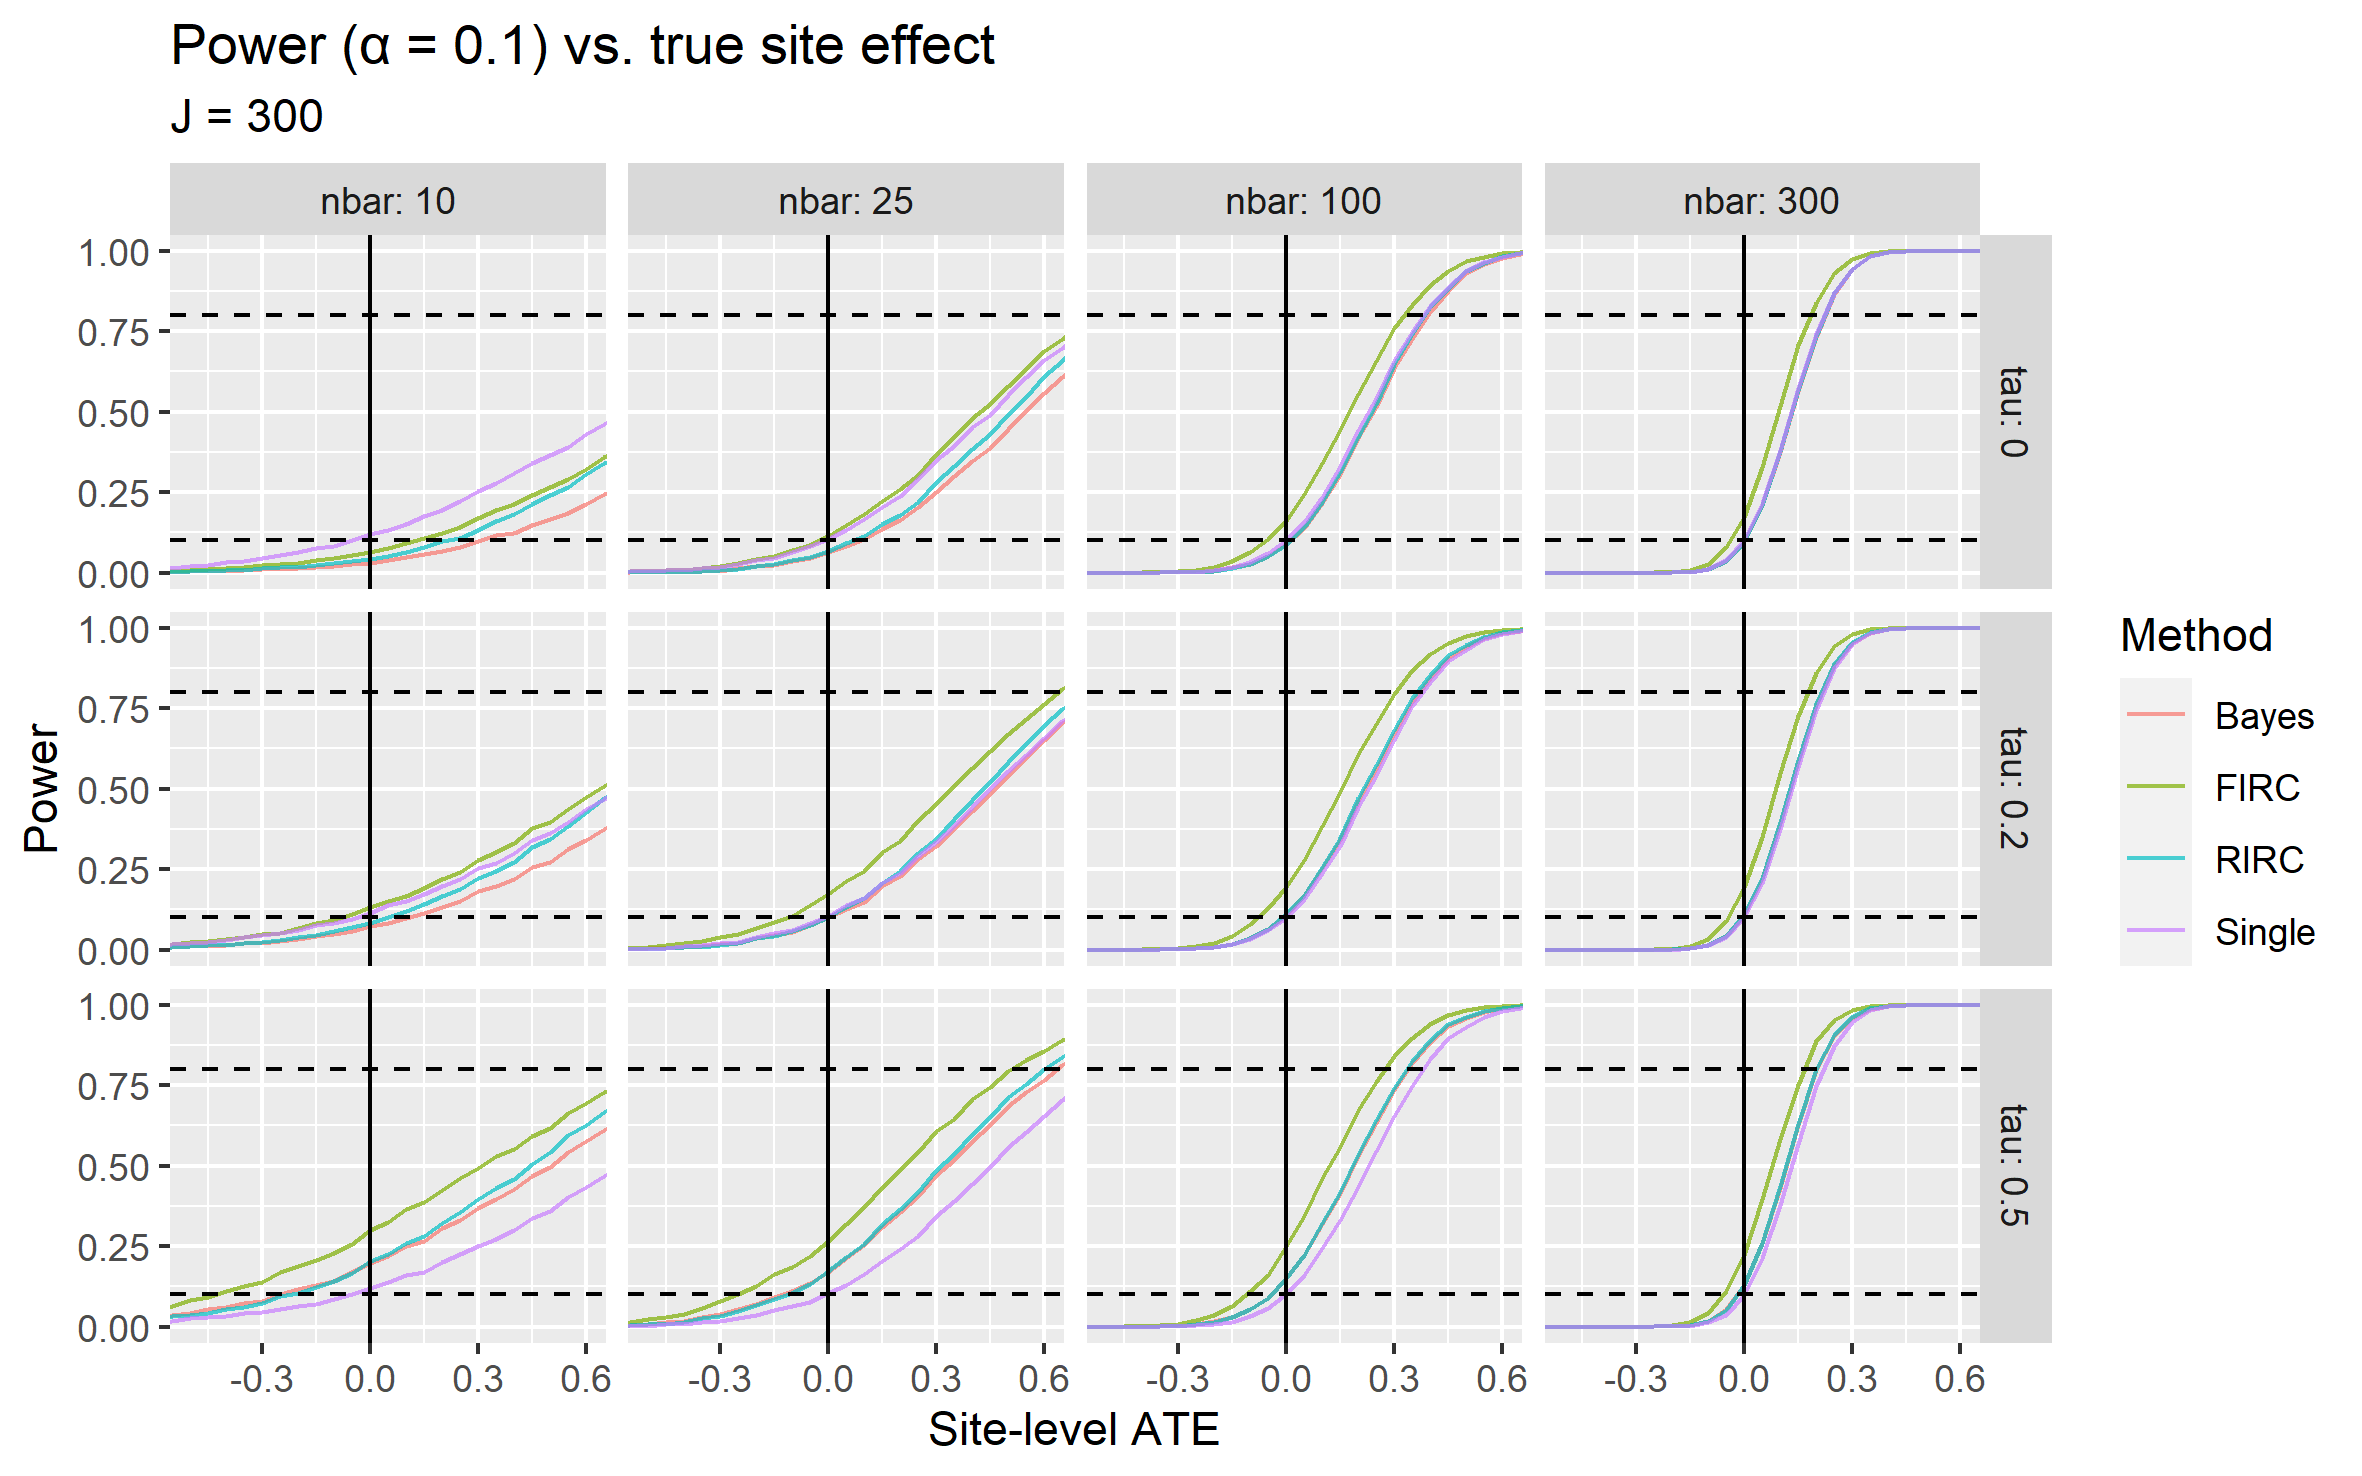
\includegraphics[width=\textwidth]{power_plot_J300}
	\caption{Plot of power (at $\alpha = 0.1$) vs. true site ATE}
	\label{fig:power_plot}
\end{figure}

To more clearly see the differences between the multilevel models and the single-site estimates, we directly plot the power differences in Figure \ref{fig:power_plot_diff}.
Positive values indicate that the MLM estimate is more powerful than the single-site estimate for the specified $\tau_j$ value.
Ideally, the curves in Figure \ref{fig:power_plot_diff} would remain below zero for $\tau_j$ values less than or equal to zero (since single-site estimates have correctly controlled false-positive rates), and would be as large as possible for $\tau_j$ values greater than zero.

\begin{figure}[ht]
	\centering
	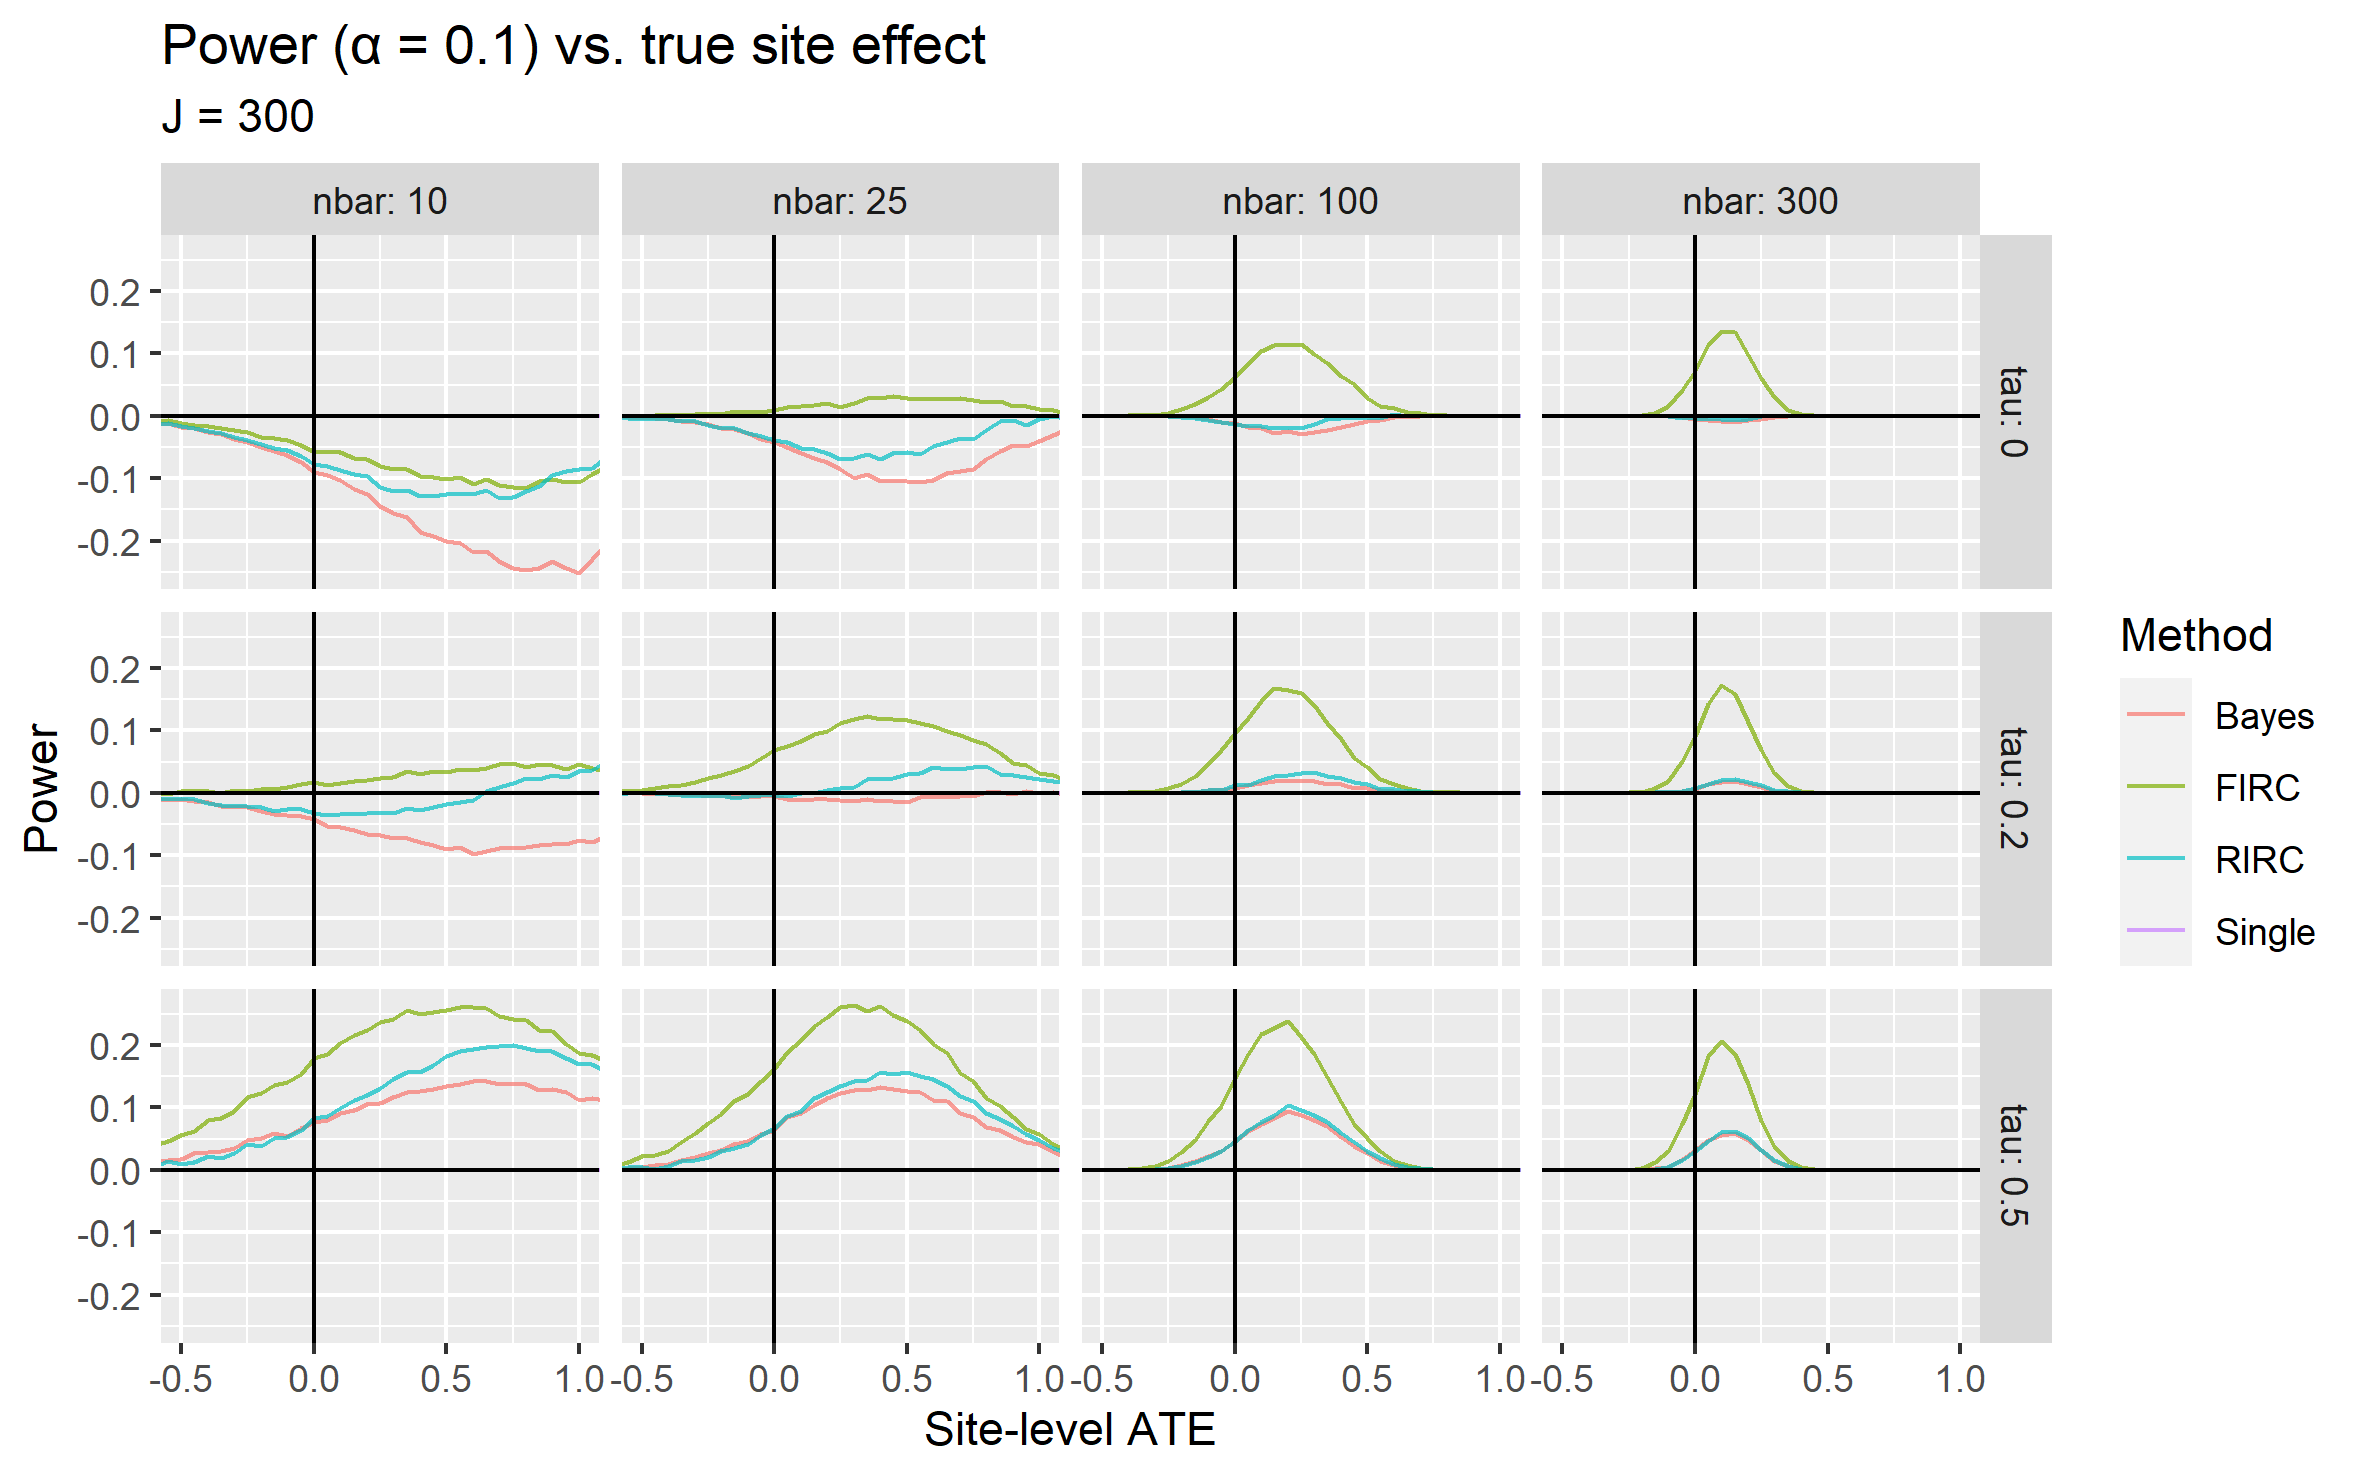
\includegraphics[width=\textwidth]{power_plot_J300_diff}
	\caption{Plot of difference in power (at $\alpha = 0.1$) between MLMs and single-site estimate vs. true site ATE}
	\label{fig:power_plot_diff}
\end{figure}

We see that overall, using MLMs provide small boosts in power, particularly for sites with small $\tau_j$ values.
Relative to the single-site estimator, the multilevel models generally have worse power when $\tau=0$ (and site estimates are shrunken toward zero) and better power when $\tau=0.5$ (and site estimate are shrunken away from zero), particularly when $\bar{n}$ is low.
Figure \ref{fig:power_plot_diff} also highlights how FIRC has much higher power than the single-site estimates for sites with small $\tau_j$ values, but that this comes at the cost of invalidity; the false positive rates for small negative $\tau_j$ values is significantly inflated.
Overall, we don't see any settings where using an MLM significantly improves power relative to the single-site estimates without inflating the false positive rate.

We can also focus on sites for which $\tau_j = 0.3$ effect-size units, which is a reasonably large effect that we would like to be able to detect in a multisite trial.
Figure \ref{fig:power_plot_ATE03} focuses on the power for these sites.
\begin{figure}[ht]
	\centering
	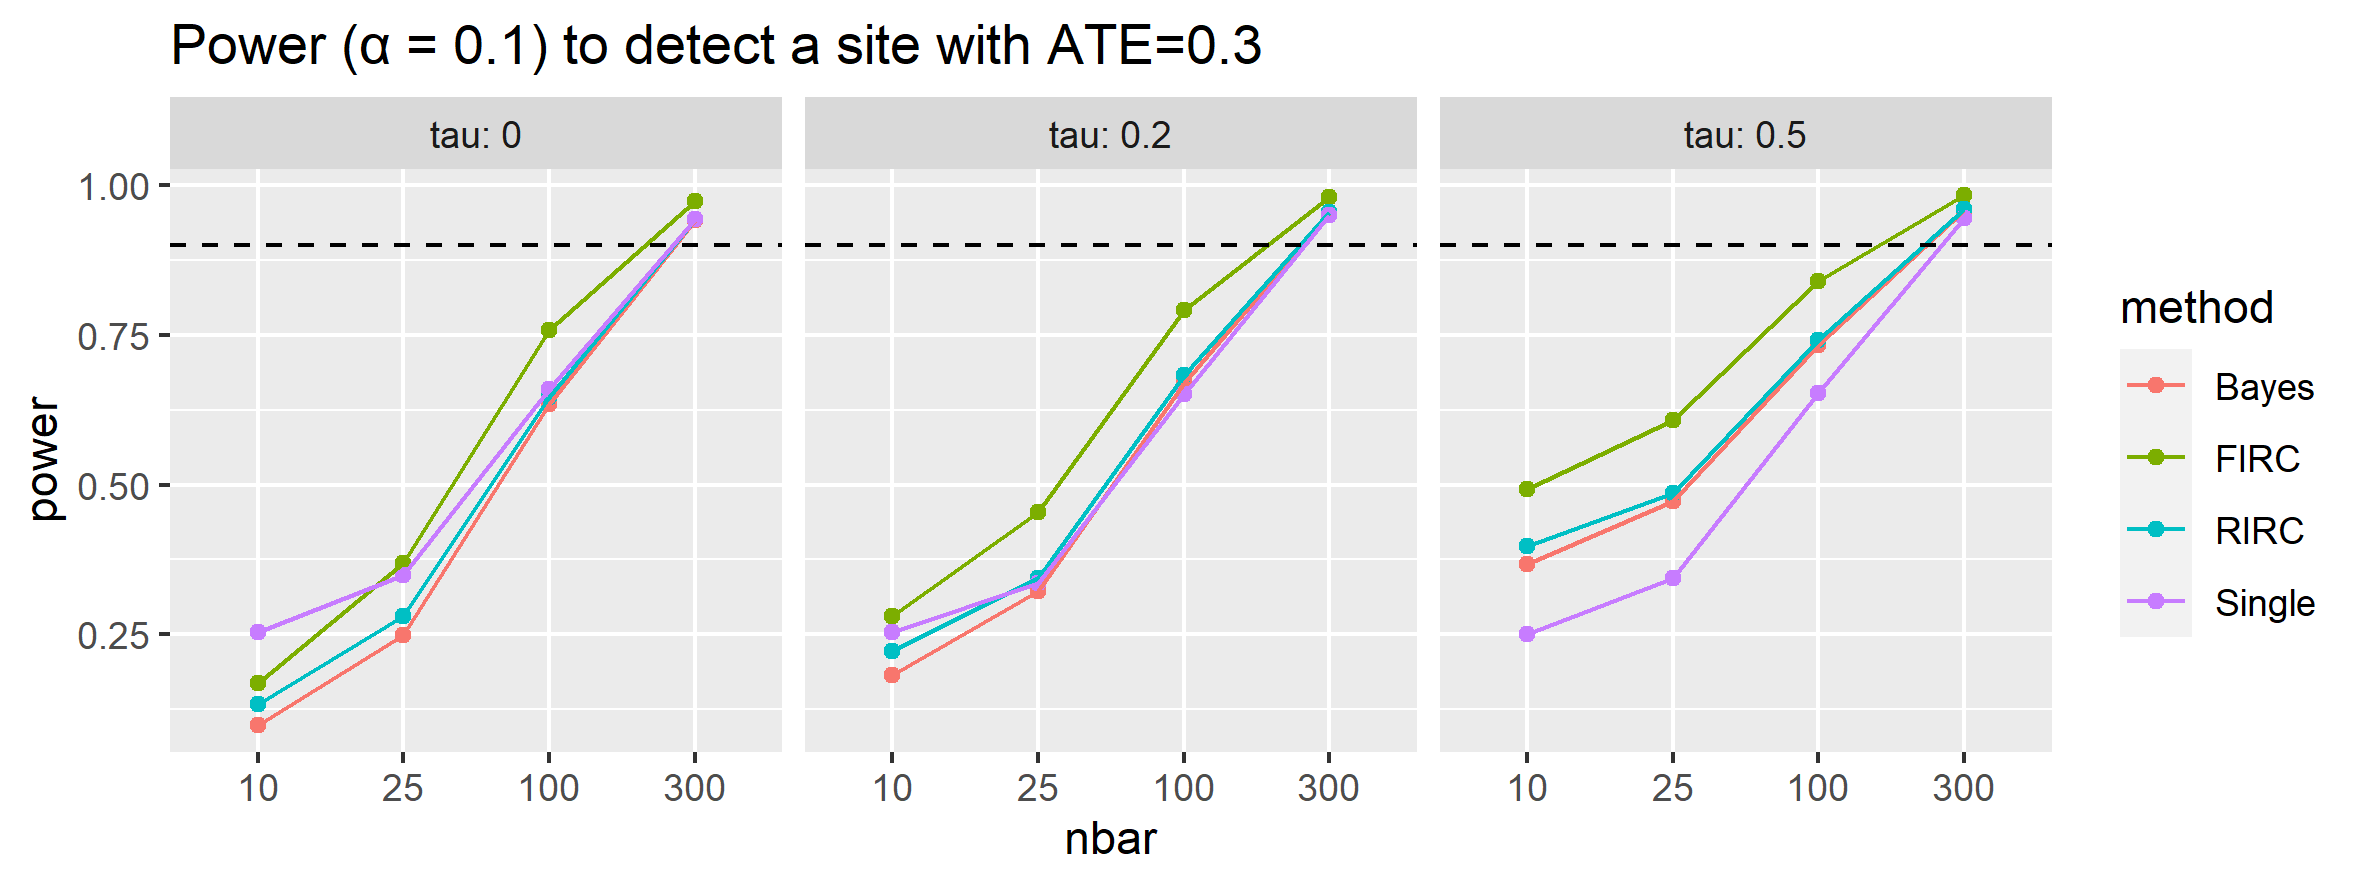
\includegraphics[width=\textwidth]{power_plot_ATE03}
	\caption{Plot of difference in power (at $\alpha = 0.1$) between MLMs and single-site estimate vs. true site ATE}
	\label{fig:power_plot_ATE03}
\end{figure}
We see that it is difficult to achieve 80\% power even when $\tau_j = 0.3$, with very low power until $\bar{n}$ exceeds 100, and that MLMs do not provide particularly large power boosts (as noted above).

To dig deeper into sites with $\tau_j = 0.3$, Figure \ref{fig:power_plot_ATE03_dens} plots density curves of estimated $\hat{\tau}_j$ values for each model when the true site effect $\tau_j = 0.2$.

\begin{figure}[ht]
	\centering
	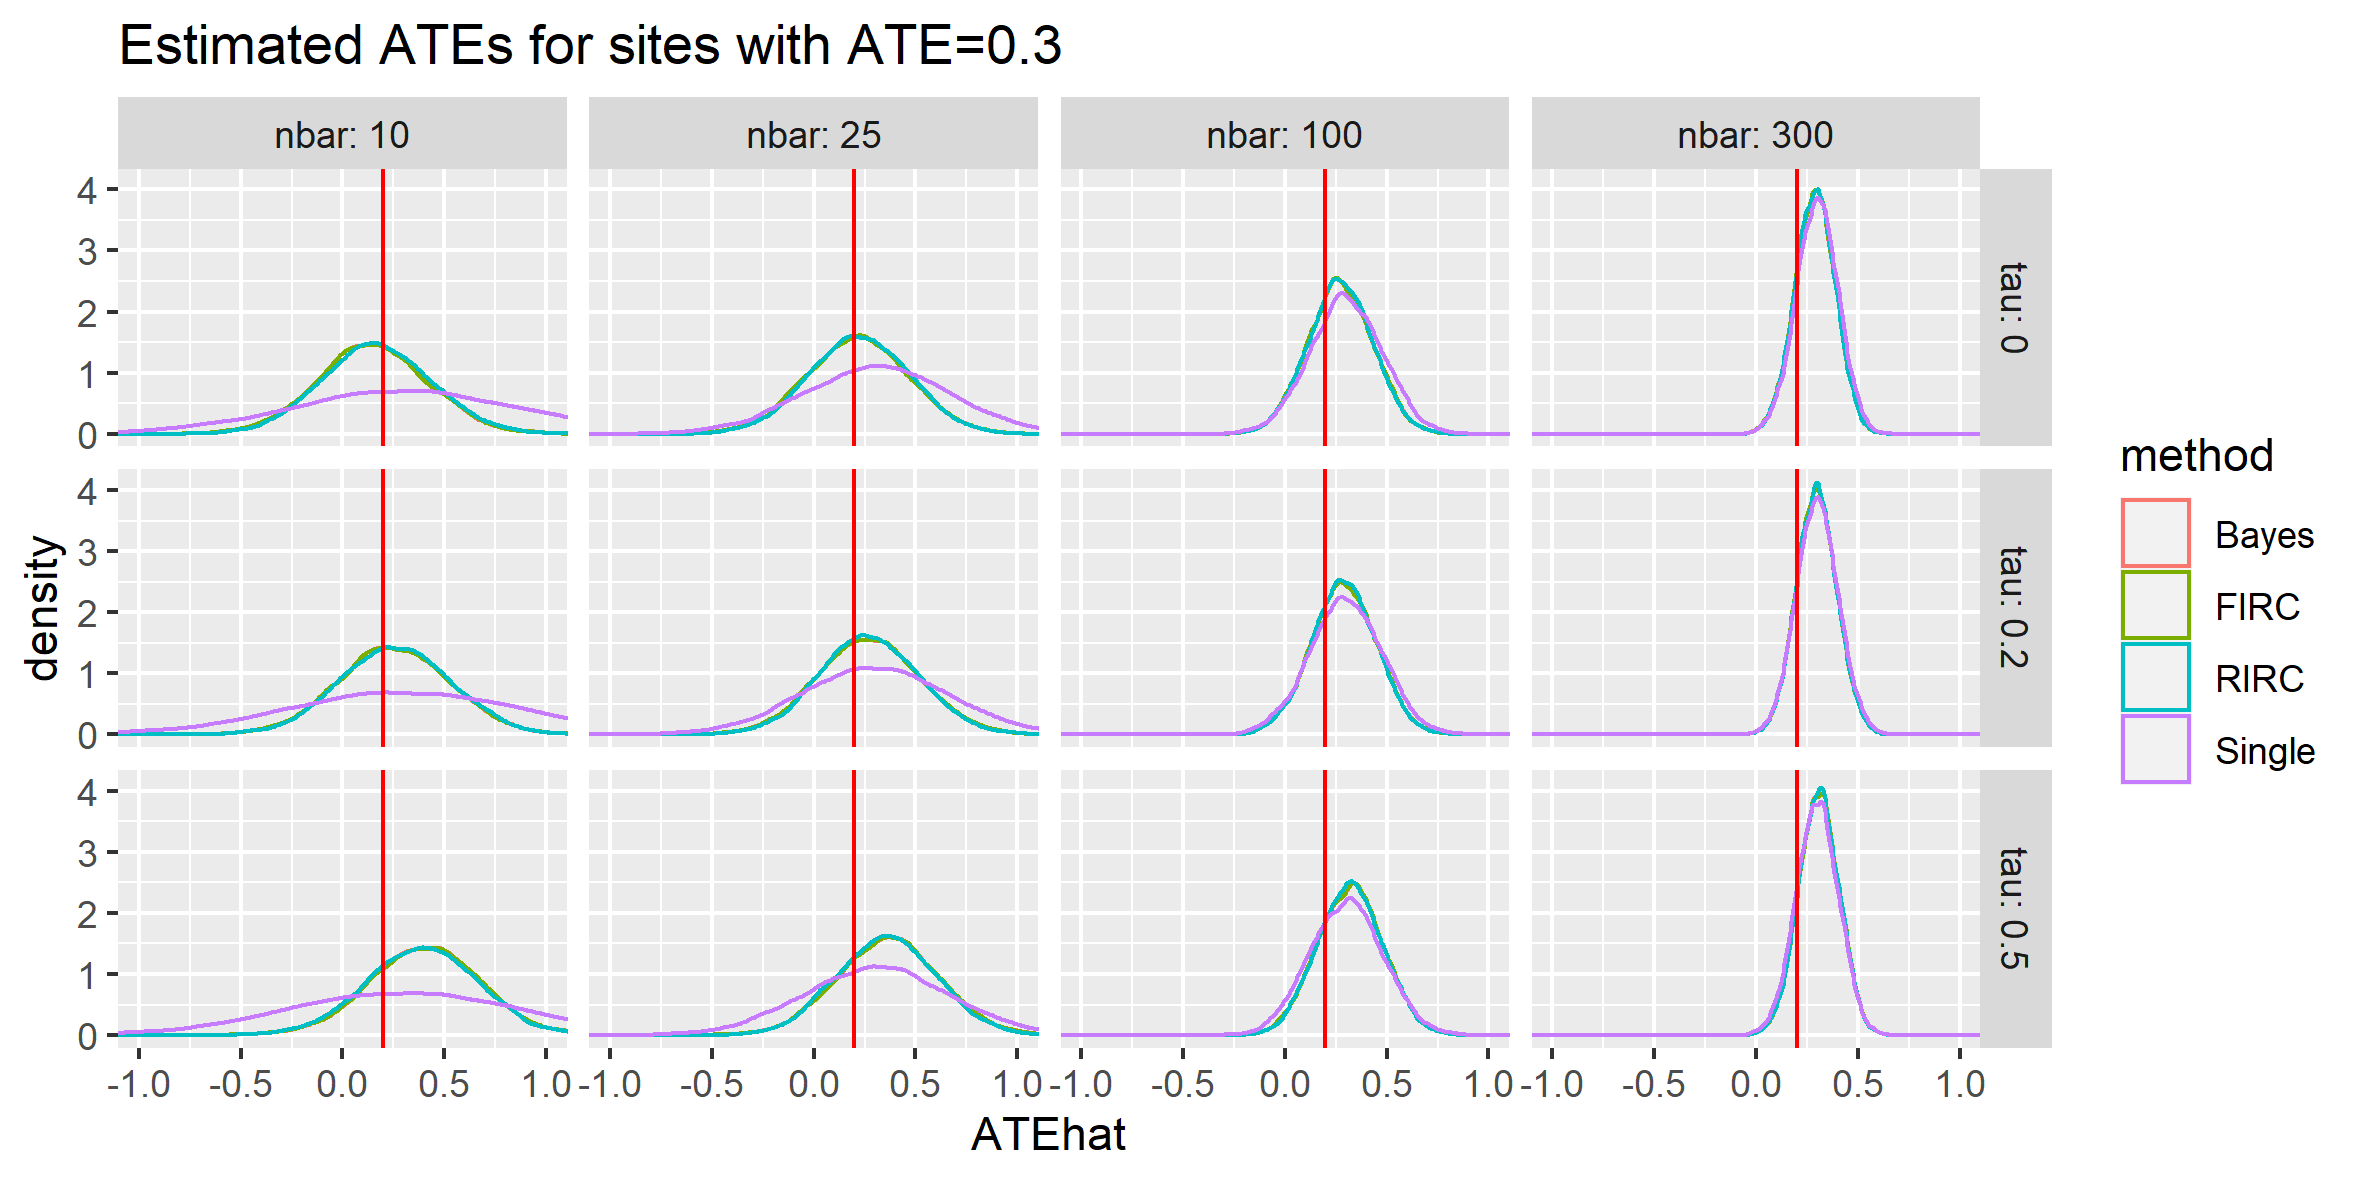
\includegraphics[width=\textwidth]{power_plot_ATE03_dens}
	\caption{Densities of estimated $\hat{\tau}_j$ values for $\tau_j = 0.2$ ($J = 50$)}
	\label{fig:power_plot_ATE03_dens}
\end{figure}

We that as $\tau$ increases, estimates get shrunken toward greater values, so the density curves shift slightly toward the right.
This shrinkage-induced bias does increase power, but at the cost of poor false positive rates and coverage for sites with $\tau_j$ far from $\tau$.
The effect disappears as the sites become more informative.

\subsection{Results: coverage}

We can also examine the coverage rates of the confidence intervals for $\tau_j$ computed under the different models.
Figure \ref{fig:coverage_plot} plots the Frequentist conditional coverage rate of 90\% two-sided confidence intervals at each true $\tau_j$ value.
We only visualize results for simulations for which $\tau = 0$.

\begin{figure}[ht]
	\centering
	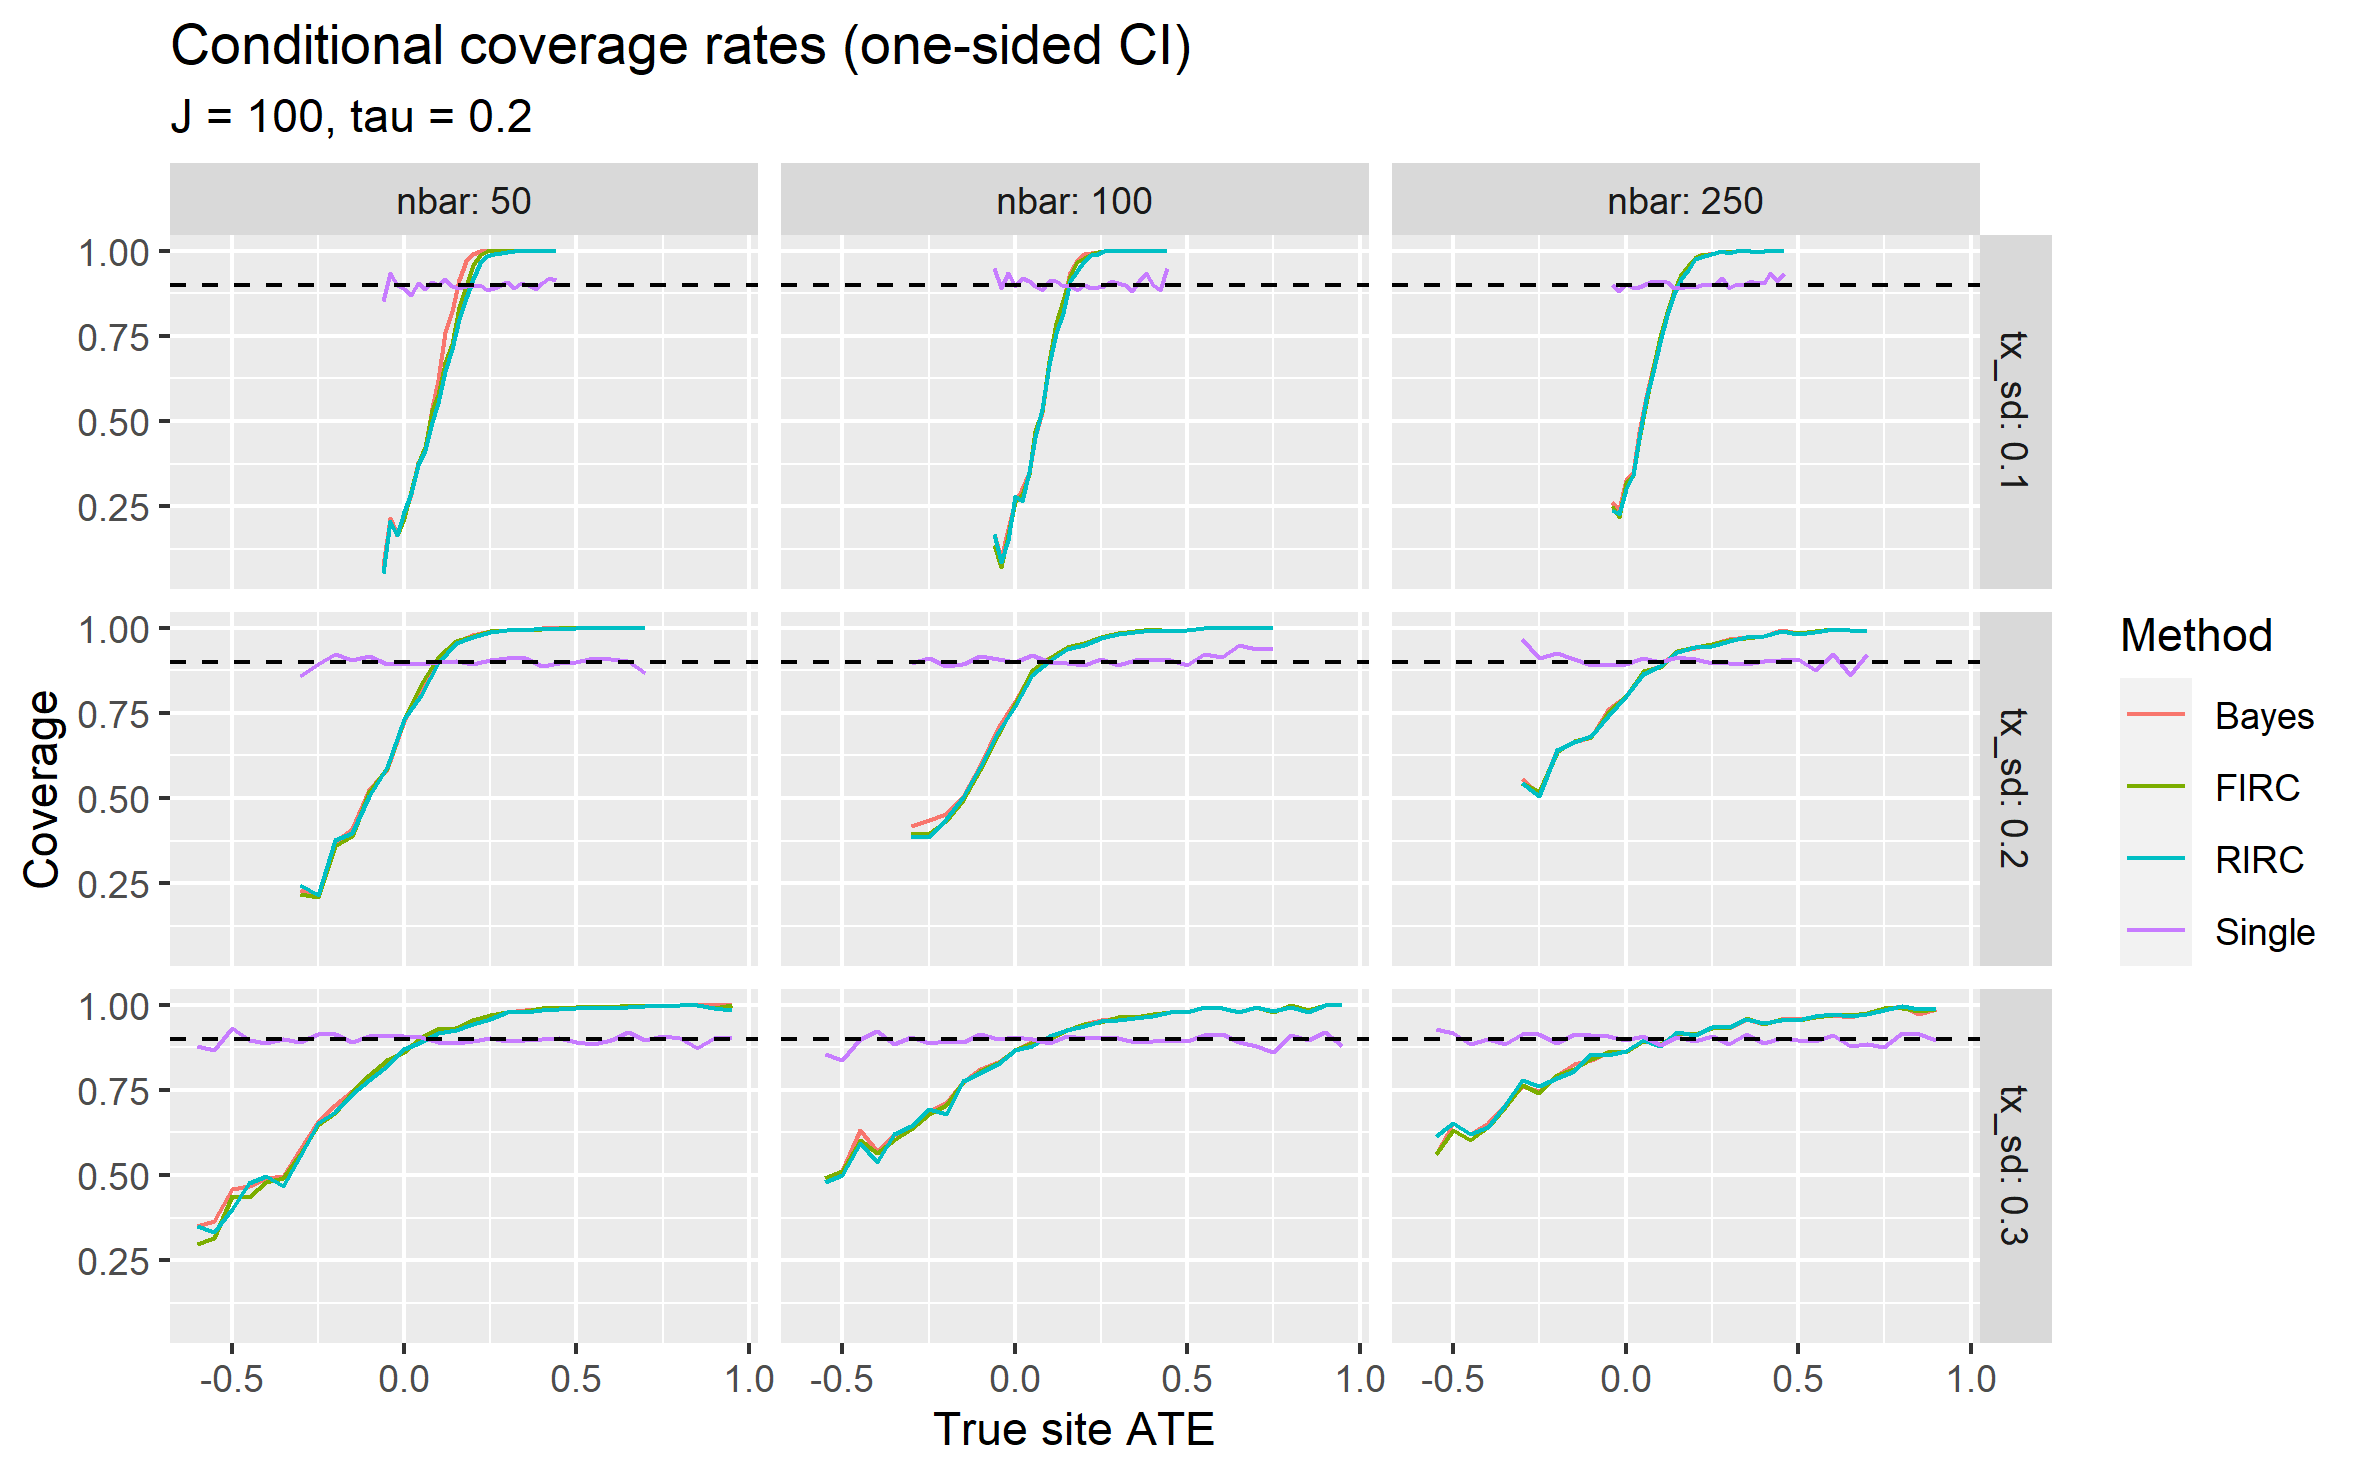
\includegraphics[width=\textwidth]{coverage_plot}
	\caption{Coverage of 90\% confidence intervals for each $\tau_j$ value}
	\label{fig:coverage_plot}
\end{figure}

The single-site estimates have roughly 90\% coverage regardless of the value of $\tau_j$ as expected, so we exclude them from the figure.
We see curvature in the coverage curves for MLMs; sites with $\tau_j$ values close to $\tau$ are overcovered, and sites with $\tau_j$ values far from $\tau$ are undercovered.
This sort of behavior is expected when examining Frequentist coverage of Bayesian procedures, where shrinkage induced by prior information (in this case, a second-level model on the $\tau_j$ values) results in overcoverage for true parameter values near the center of shrinkage at the cost of undercoverage for parameter values far from the center of shrinkage.
The curvature in the coverage curve is the most extreme when sites are uninformative (e.g., smaller, so that the model does a significant amount of shrinking), and it becomes less extreme as the sites grow more informative (e.g., larger).

Three features jump out when comparing results for the Bayes, FIRC, and RIRC models.
First, we see that the FIRC model consistently undercovers.
This is unsurprising because we follow the standard practice of only using the standard error of the estimated random residual $\tau_j - \tau$, and not also adding in the standard error of the estimate of $\tau$.
It is somewhat more surprising that the RIRC model can be approximately correct even without incorporating the standard error of the estimate of $\tau$.
Second, we confirm that as $\bar{n}$ increases, the EB estimates from the three models all approach the single-site estimates, so their coverage curves naturally become flatter.
Finally, we see that increasing $J$ appears to improve the average coverage of the FIRC and RIRC models, while having little effect on the fully Bayesian model.
It's not very clear why this should be the case, though presumably it should have to do with improved cross-site variance estimation as $J$ increases.

We can also visualize the EB coverage of the different methods.
Figure \ref{fig:EBcoverage_plot} shows the results for $\tau=0$ (the other values of $\tau$ produce the same results).

\begin{figure}[ht]
	\centering
	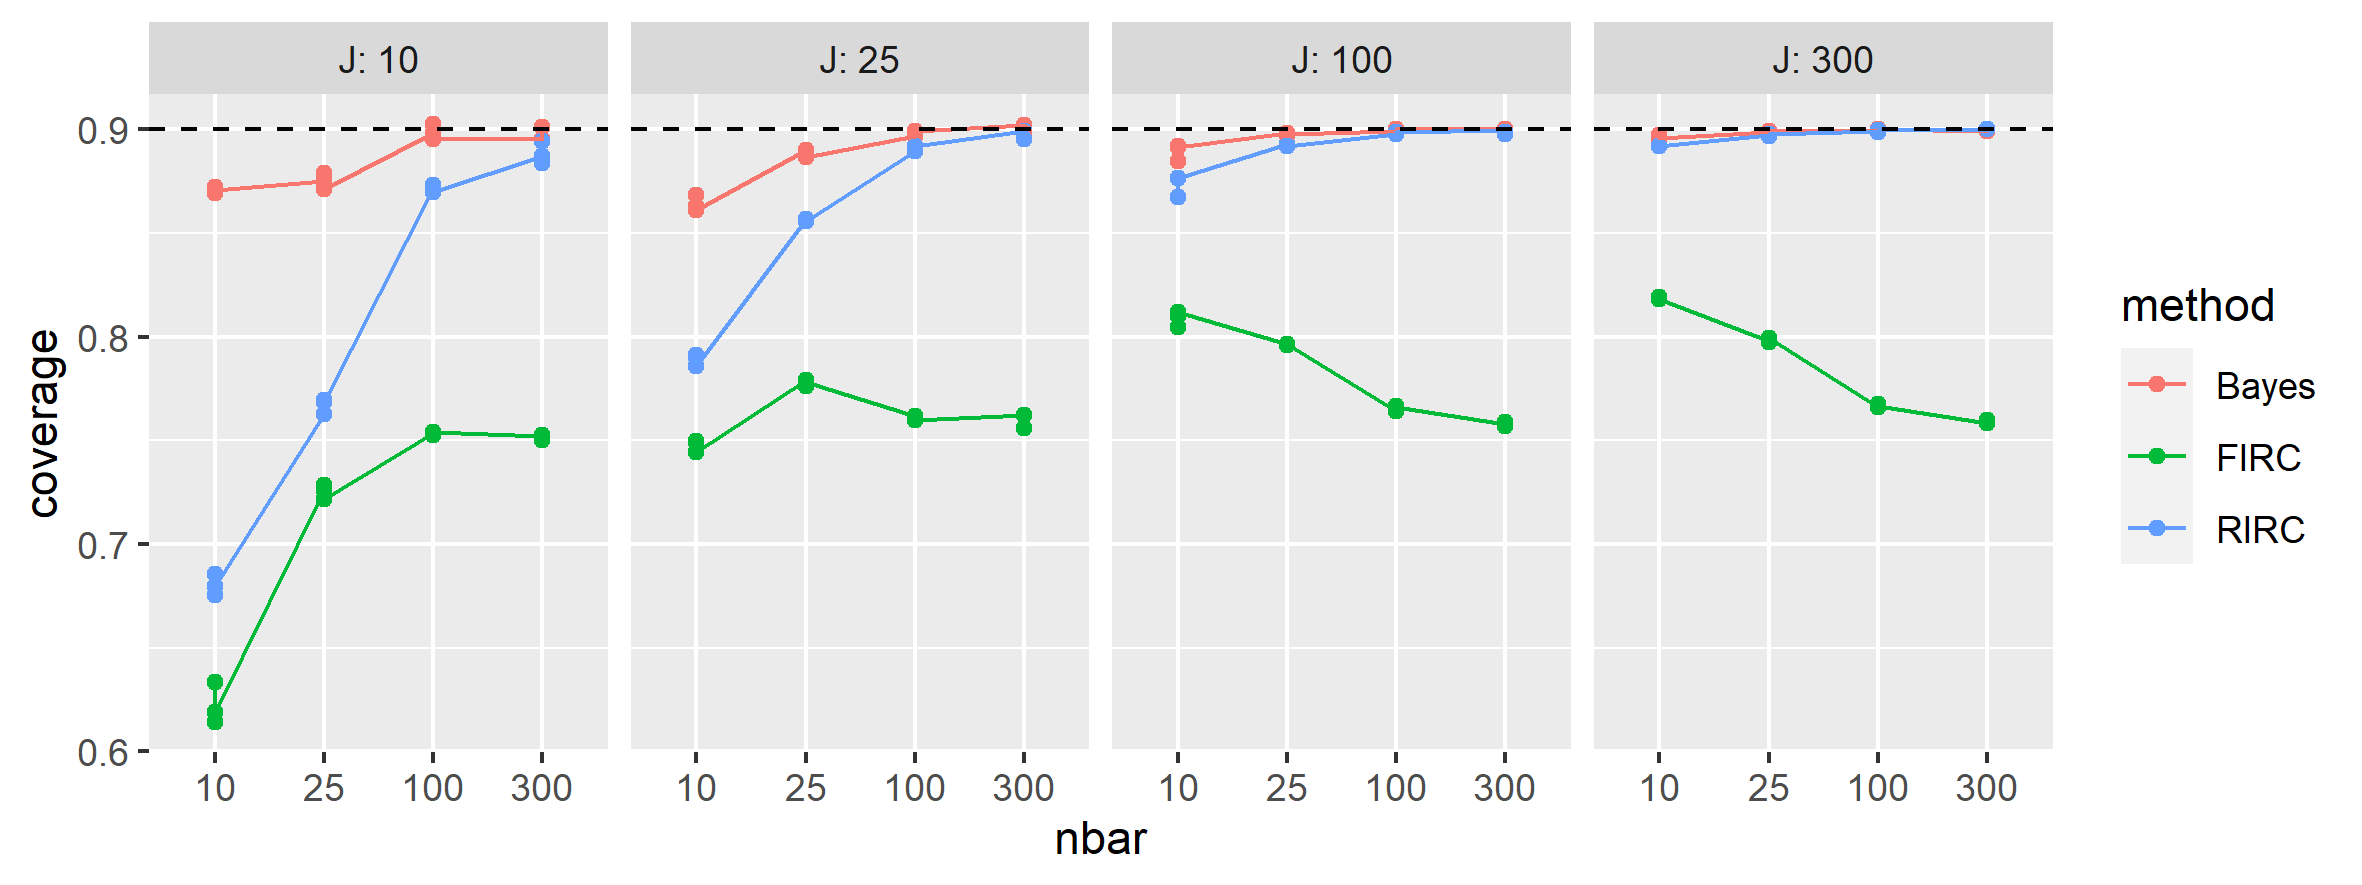
\includegraphics[width=\textwidth]{coverage_plot_eb}
	\caption{Empirical Bayes coverage of 90\% confidence intervals, $\tau=0$}
	\label{fig:EBcoverage_plot}
\end{figure}

The FIRC model seriously undercovers, as we saw before.
Interestingly, the fully Bayesian and RIRC models have better EB coverage than the single-site estimates when $\bar{n}$ is low but $J$ is high; here, pooling information across sites actually improves EB coverage.
Also, we again see the RIRC model's serious undercoverage in the low-information cases, unlike the fully Bayesian model, which always covers at least as well as do the single-site estimates.

\subsection{Results: Root-mean-squared error (RMSE)}

As a sidebar, we can confirm that using MLMs improves the RMSE of the collection of site-effect estimates, where RMSE is defined as:
$$RMSE = \sqrt{\frac{1}{J} \sum_{j=1}^J (\hat{\tau}_j - \tau_j)^2}.$$
Figure \ref{fig:rmse_plot} shows the RMSEs of our estimators across our 1000 simulation runs.
We see that using MLMs indeed decreases RMSE as expected, with the decrease being largest for uninformative sites.
Interestingly, the RIRC model seems to perform marginally better than the other models in terms of RMSE.

\begin{figure}[ht]
	\centering
	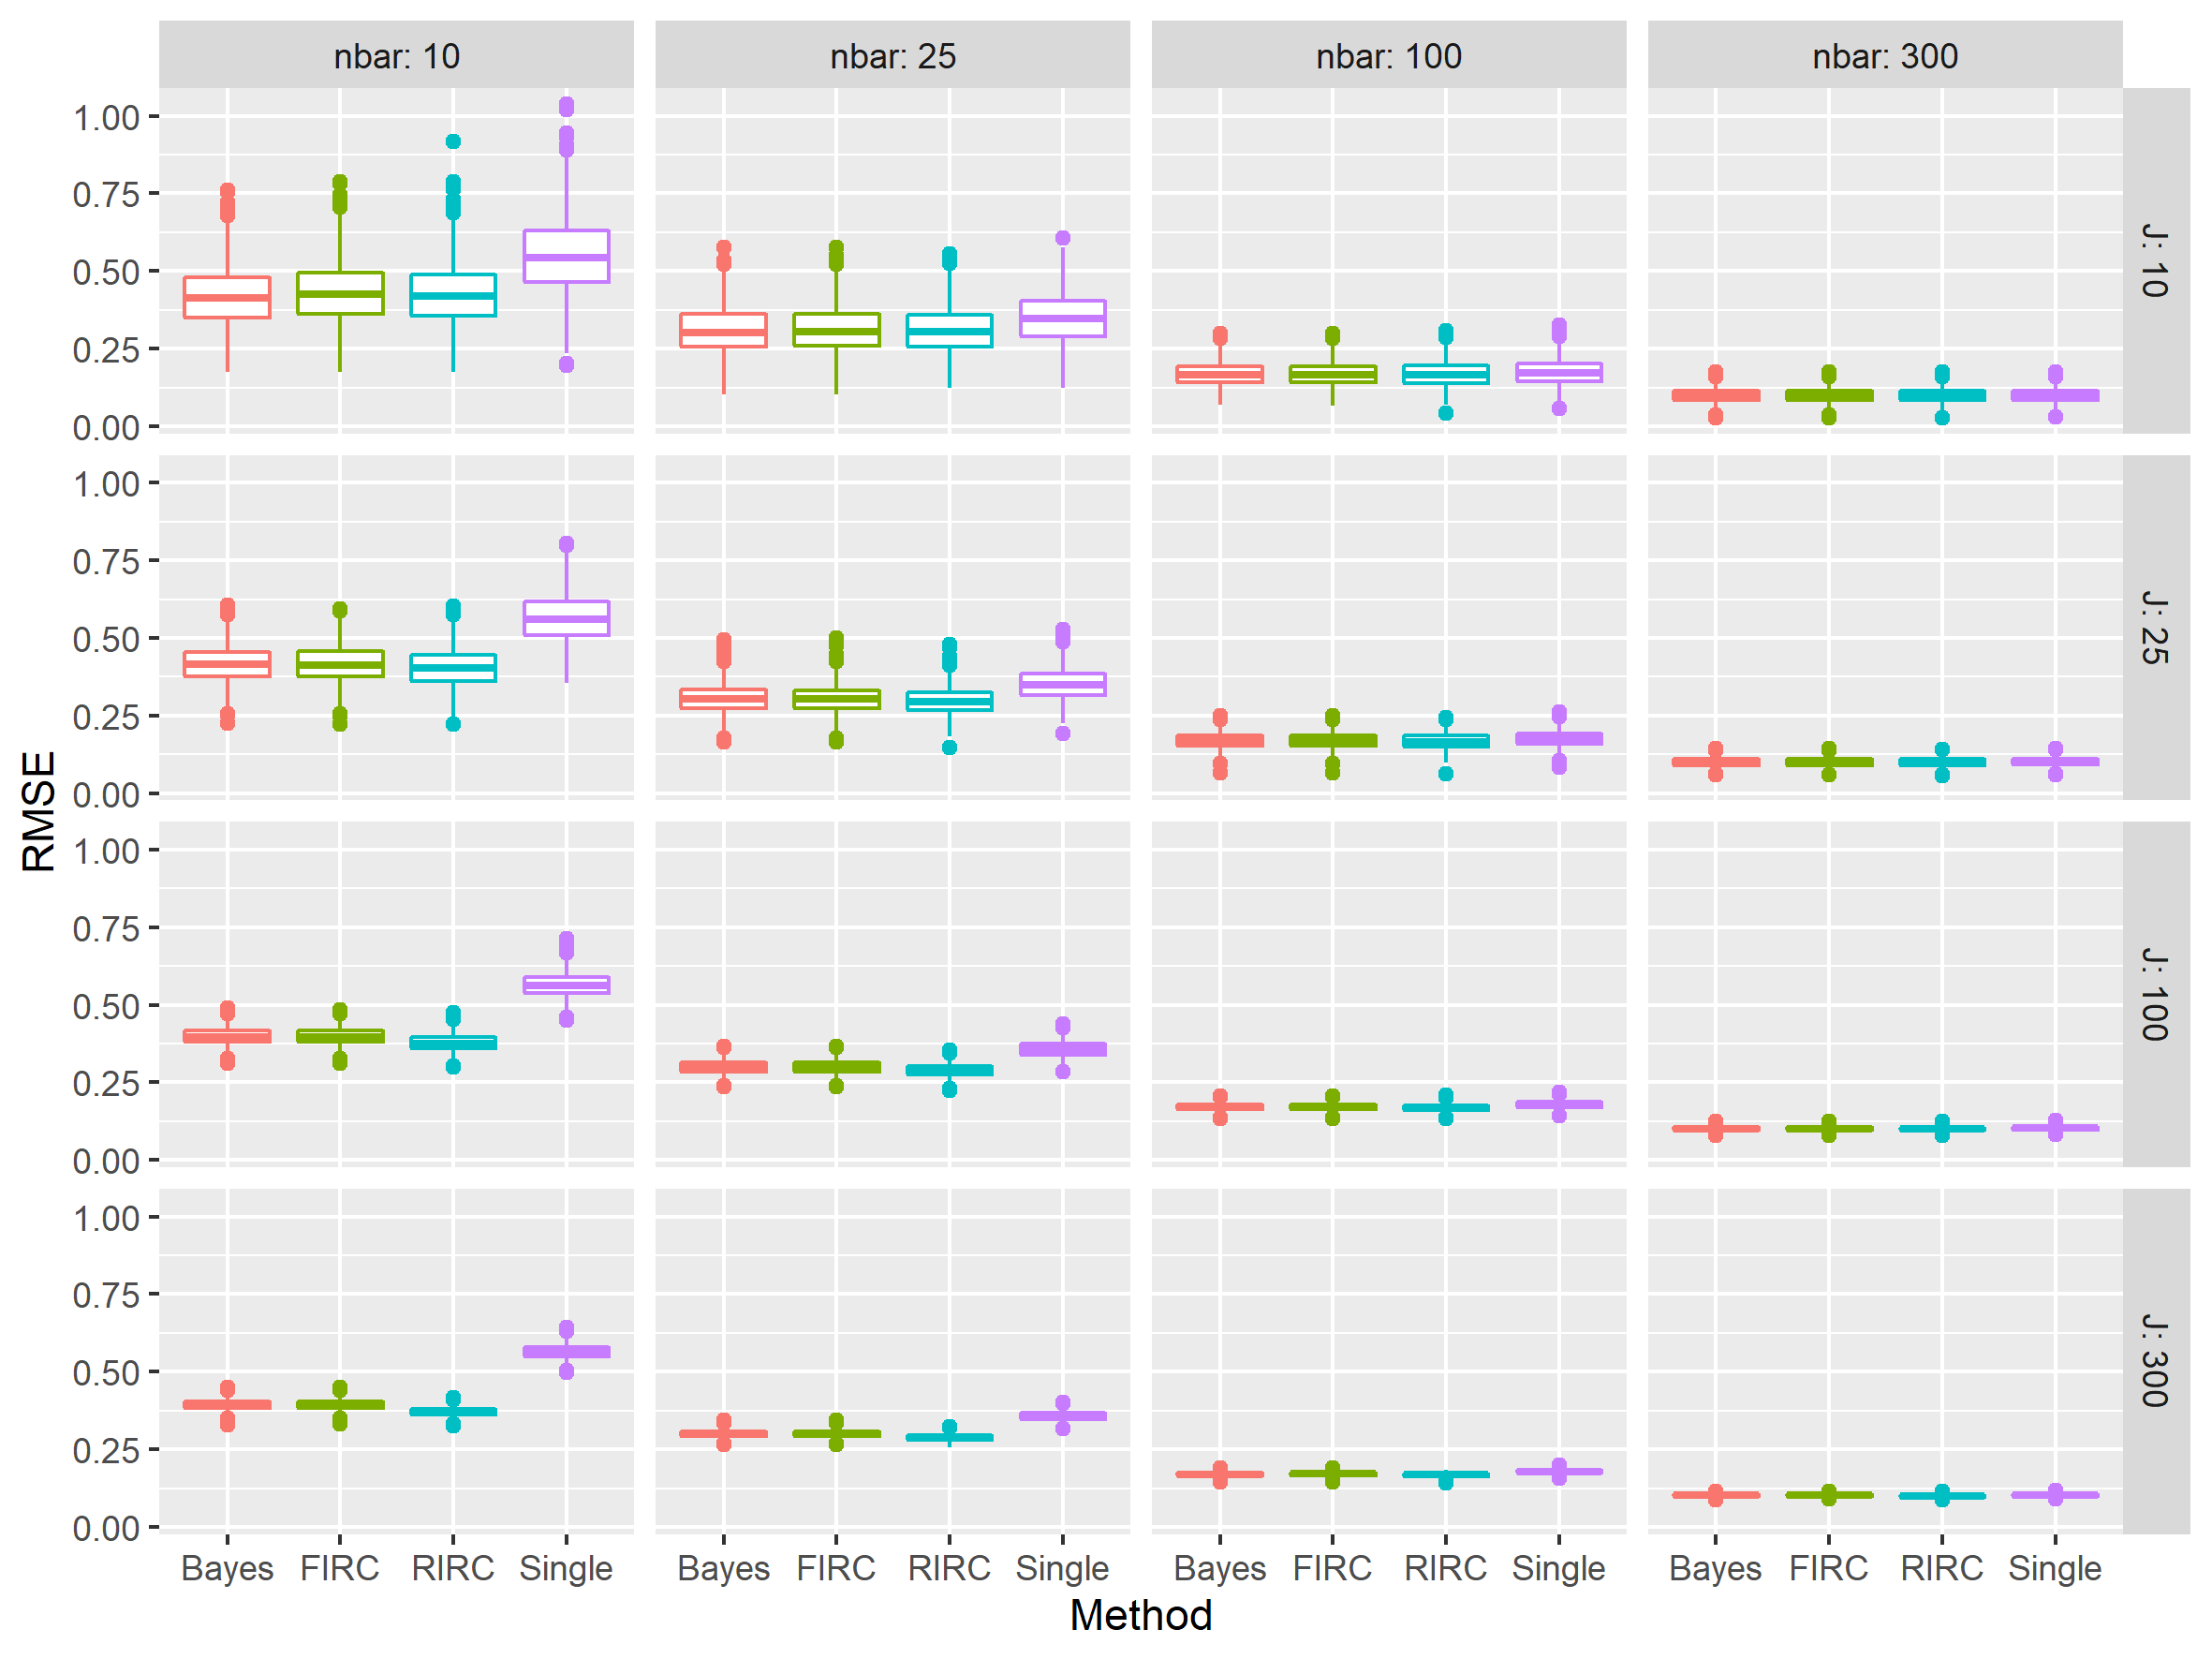
\includegraphics[width=\textwidth]{rmse_plot}
	\caption{Root-mean-squared error of site effect estimates}
	\label{fig:rmse_plot}
\end{figure}

\section{Case study: example power analysis}

\subsection{Power analysis setup}

In this section, we perform an example power analysis.
Suppose we have a setting with $J=20$ sites, and we'd like to know how many students per site (on average) we'd need to identify various single-site effects, i.e., we would like to understand how single-site power varies as a function of $\bar{n}$.
We might also be interested in the power to detect an overall effect.

To run this power analysis, we assume that $ICC=0.2$ and $\tau=0.2$.
We further assume that the data-generating process is as defined in our simulation study, and treatment variation is 0.3.
We then repeatedly simulate data under these conditions and estimate both power to detect $\tau > 0$ and power curves for detecting $\tau_j > 0$.
If we only had one particular $\tau_j$ value we were interested in, we could use set-site simulation here; for now, we'll continue with all-site simulation to get power curves.

\subsection{Power analysis results}

Figure \ref{fig:power_plot_ex} shows how power varies as a function of site size, for true site-level effects of $\tau_j = 0.2, 0.3, 0.4$.
\begin{figure}[ht]
	\centering
	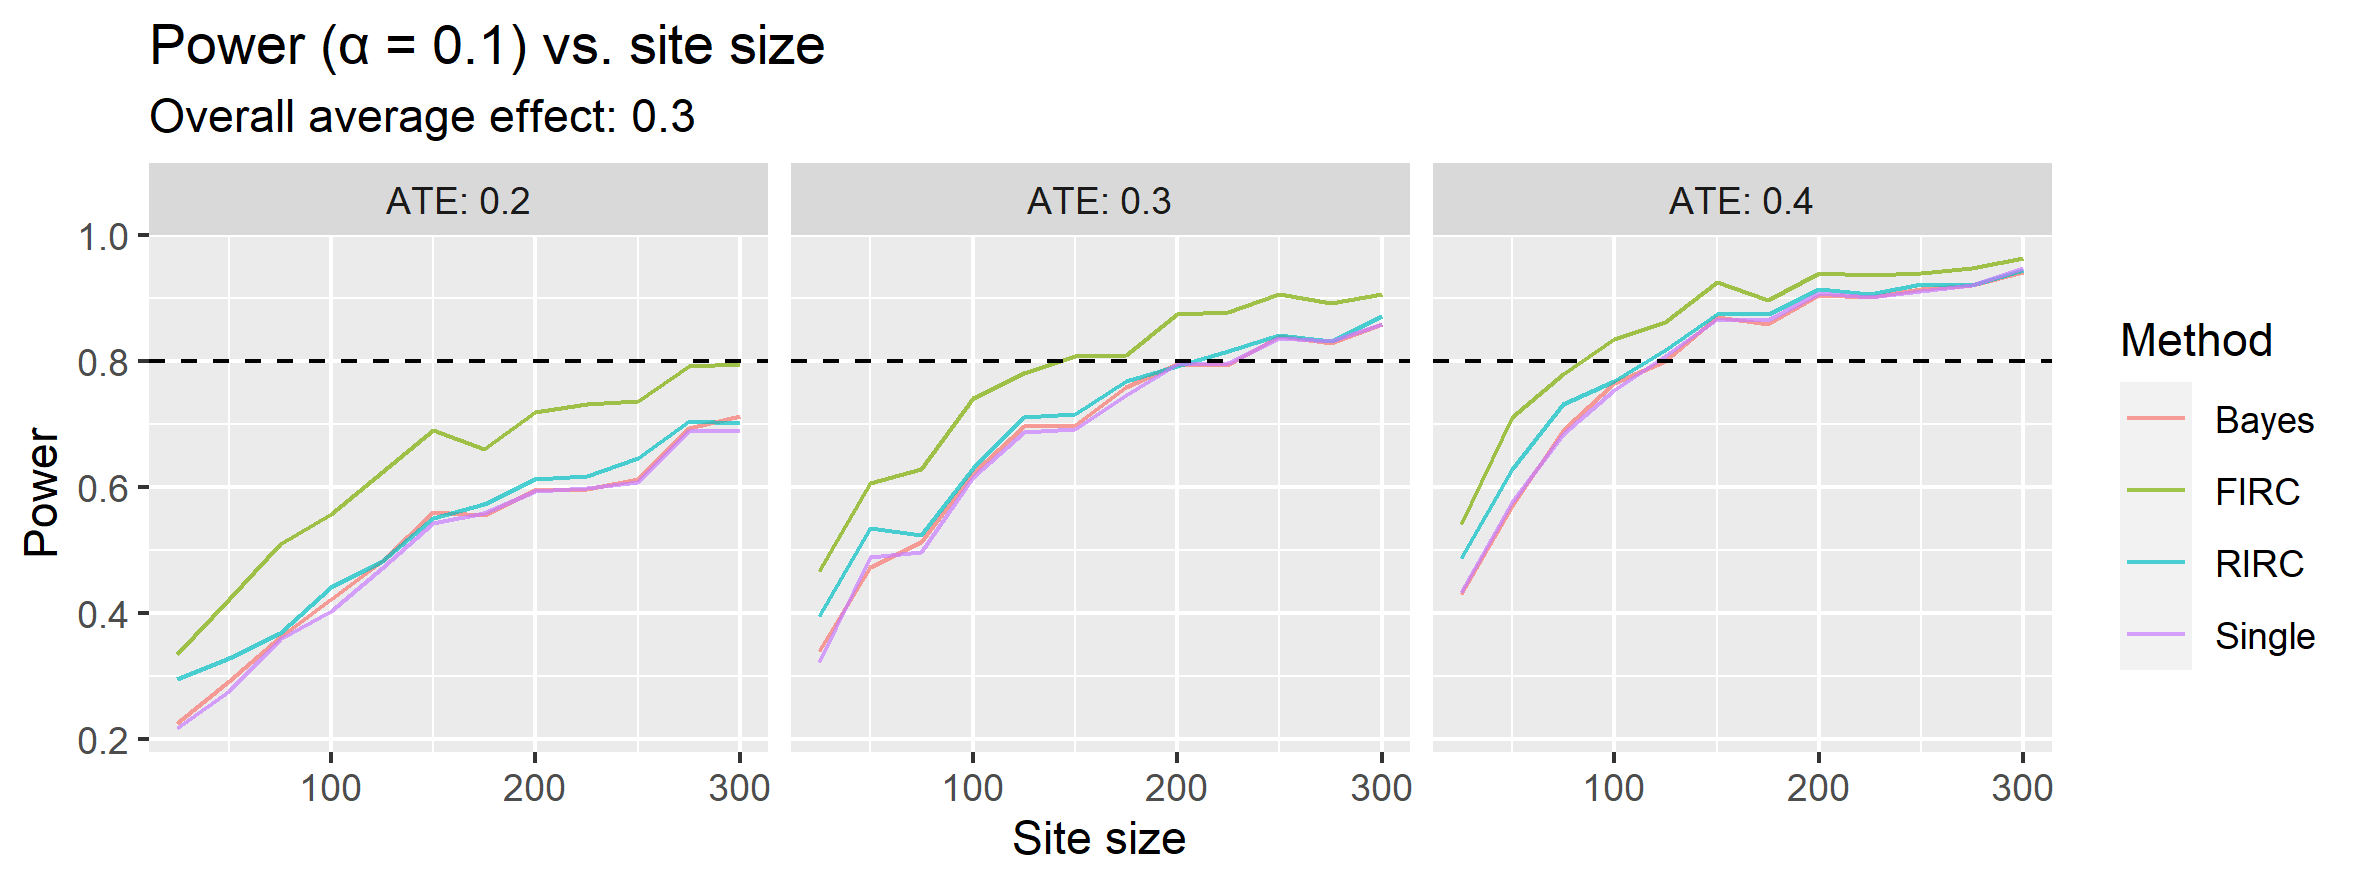
\includegraphics[width=\textwidth]{power_plot_ex}
	\caption{Power curve for site-specific effect}
	\label{fig:power_plot_ex}
\end{figure}
As expected, power increases with the sizes of the individual sites.
We see that it is difficult to consistently detect sites with site-level effects of $\tau_j = 0.2$, even when each site has 300 observations.
As $\tau_j$ increases, it becomes easier to detect the site-level effect.

Figure \ref{fig:power_plot_overall} plots (one-sided test) power for detecting an overall effect, at $\alpha = 0.1$.
\begin{figure}[ht]
	\centering
	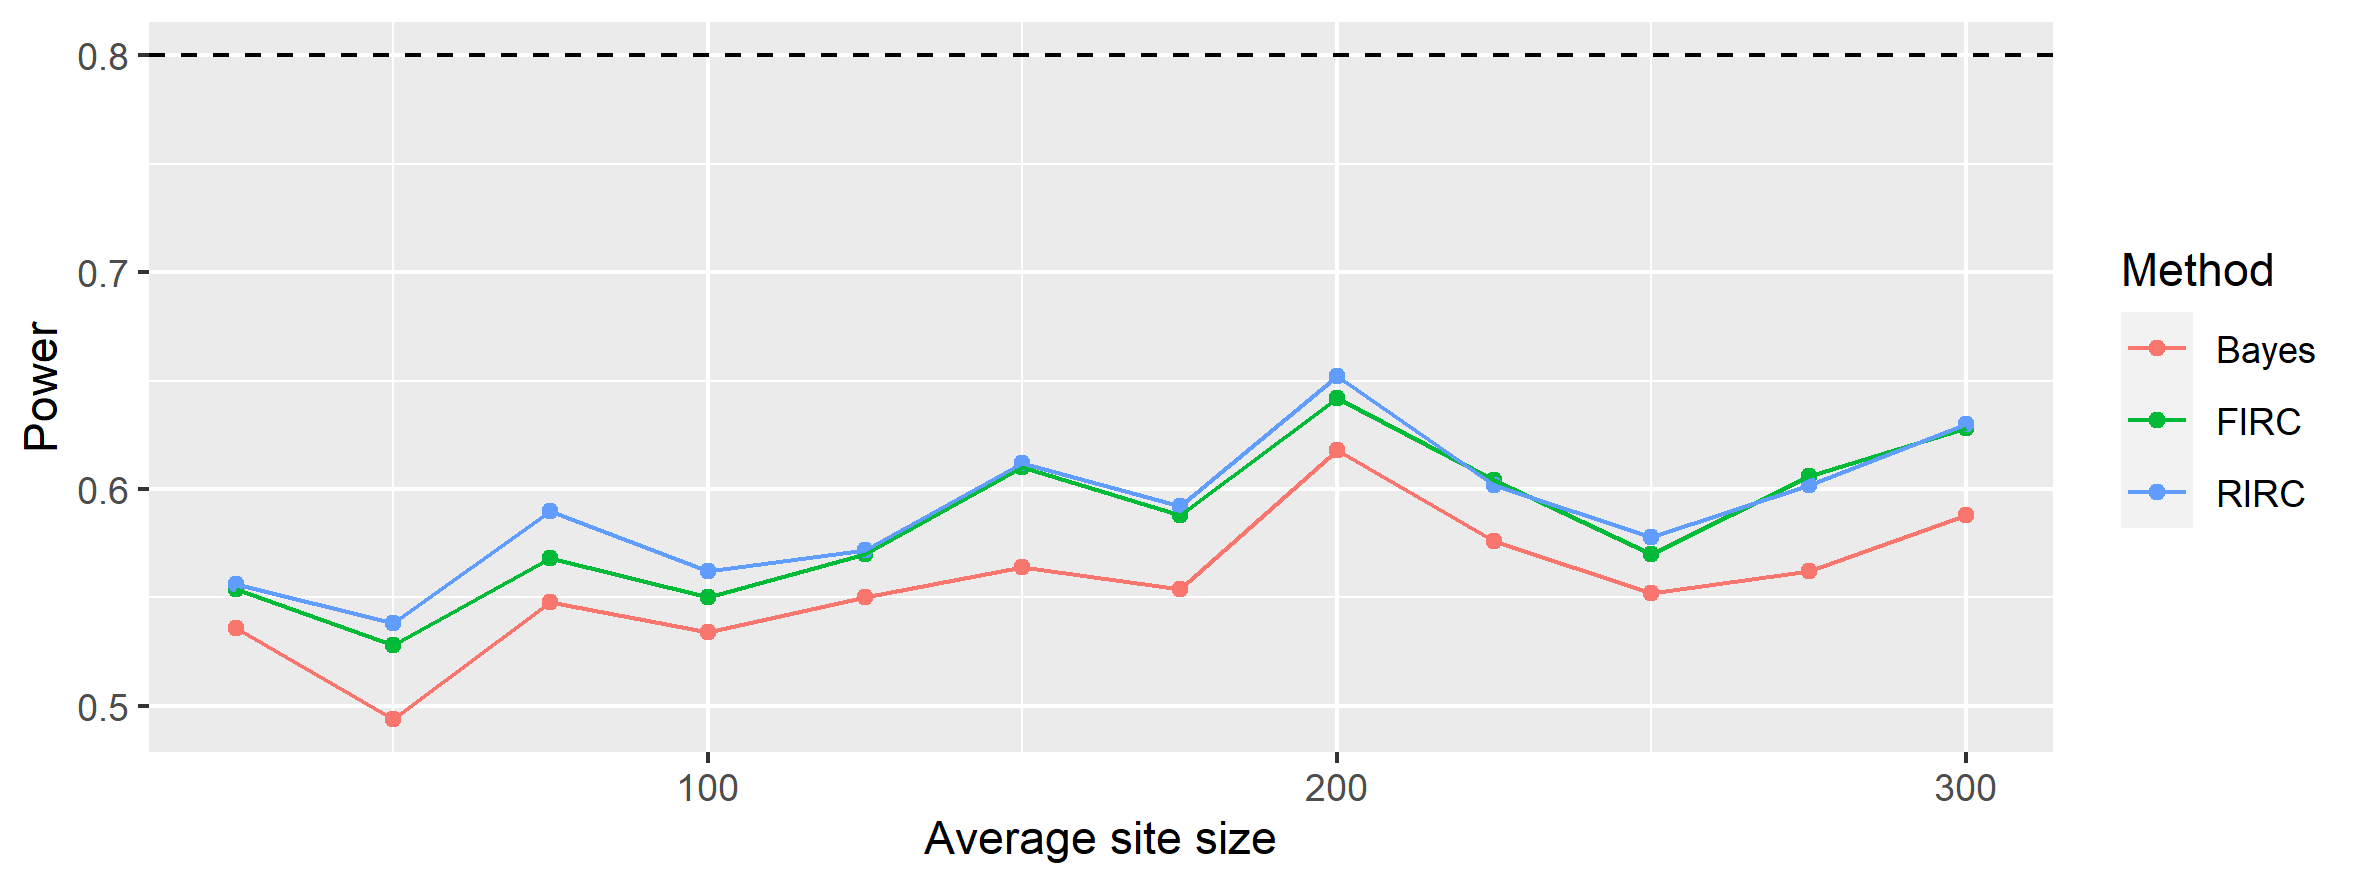
\includegraphics[width=\textwidth]{power_plot_overall_tau02}
	\caption{Power curve for overall effect}
	\label{fig:power_plot_overall}
\end{figure}
In our case with $J=20$ sites, even an average of 300 observations per site is insufficient for 80\% power to detect the overall effect.
FIRC and RIRC have slightly more power here, but as Figure \ref{fig:coverage_plot_overall} shows, they have slightly suboptimal coverage.
It is not clear to me why this occurs, but regardless, we can note that it does, so we should be slightly cautious about interpreting the FIRC/RIRC intervals for $\tau$ in this $J=20$ case.

\begin{figure}[ht]
	\centering
	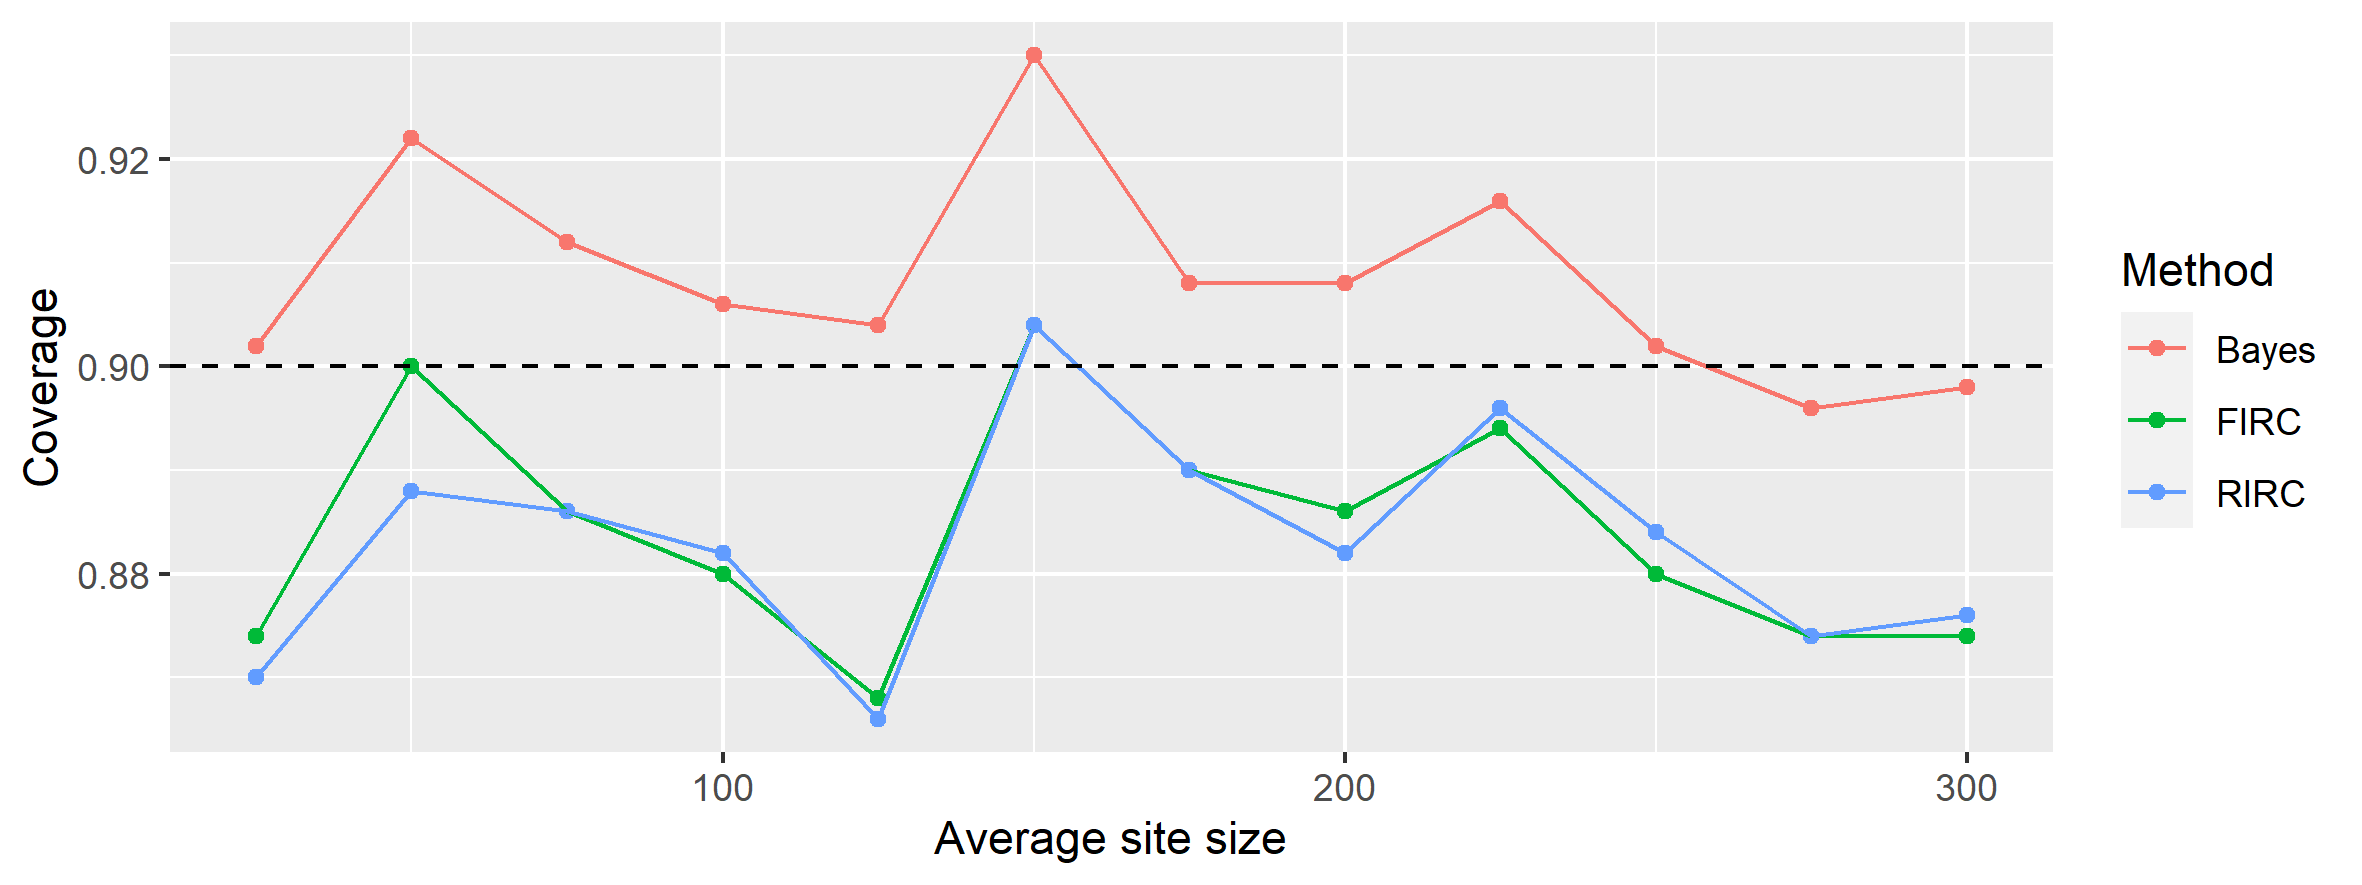
\includegraphics[width=\textwidth]{coverage_plot_overall_tau02}
	\caption{Coverage curve for overall effect}
	\label{fig:coverage_plot_overall}
\end{figure}


\section{Discussion}

Overall, MLM shrinkage marginally increases rejection rates, relative to single-site estimates.
The increase in power, however, is not particularly strong, and often comes with inflated false positive rates and poor coverage properties.
When comparing different MLMs, we saw that while the FIRC model rejects the null more frequently than the RIRC and fully Bayesian models, it does so at the cost of an inflated type-I error rate.
Similarly, the RIRC model exhibits slightly higher power in certain scenarios at the cost of poor coverage in low-data settings, though its coverage is not nearly as bad as the FIRC model's coverage.
Finally, while the fully Bayesian model always has approximately appropriate coverage, it only improves power when $\tau$ is high (and $\tau_j$ estimates are biased upward), and significantly decreases power when $\tau$ is low.

Ultimately, this simulation study shows that MLMs do not really help to improve point estimates or inferences for treatment effects at individual sites.
While MLMs certainly improve estimates for the full collection of site estimates in terms of RMSE, this does not imply better estimates for any particular site (a la Stein's paradox\footnote{Stein's paradox notes that when estimating three or more parameters at the same time, it is possible to construct an estimator that is better for the collection of all three parameters, in terms of average MSE, than any estimator that estimates the three parameters separately.
This, however, does not imply that the new estimator is better for any individual parameter.}).
Practitioners interested in improving power to detect effects at individual sites should aim to make the individual site's estimate more precise, rather than aiming to add other sites to the analysis.

\appendix
\section{Appendix A: model details}

The FIRC model assumes a fixed intercept per site, but a random coefficient on the site-level treatment effects:
\begin{align*}
	Y_{ij} &= \alpha_j + \tau_j Z_{ij} + \epsilon_{ij} \\
	\tau_j &= \tau + u_{1j} \\
	u_{1j} &\sim N(0, \sigma^2_\tau) \\
	\epsilon_{ij} &\sim N(0, \sigma^2_y).
\end{align*}
Technically, the FIRC model allows for separate variance parameters $\sigma^2_{y 1}$ and $\sigma^2_{y 0}$ for the treated and control groups.
Since our data-generating procedure just uses a single $\sigma^2_y$ for both the treatment and control groups, we opt to use the simpler model shown above.

The RIRC model instead assumes a random intercept per site:
\begin{align*}
	Y_{ij} &= \alpha_j + \tau_j Z_{ij} + \epsilon_{ij} \\
	\alpha_j &= \alpha + u_{0j} \\
	\tau_j &= \tau + u_{1j} \\
	\begin{pmatrix}
		u_{0j} \\ u_{1j}
	\end{pmatrix} &\sim N\left(
	\begin{pmatrix}
		0 \\ 0
	\end{pmatrix}, 
	\begin{bmatrix}
		\sigma^2_\alpha & \rho_{01} \\  & \sigma^2_\tau
	\end{bmatrix}\right) \\
	\epsilon_{ij} &\sim N(0, \sigma^2_y) ,
\end{align*}

The fully Bayesian model is fit to the site-level effect estimates $\hat{\tau}_j$ and (estimated) standard errors $se(\tau_j)$.
It places a half-Normal prior on $\sigma^2_\tau$, and a diffuse Normal prior on $\tau$:
\begin{align*}
	\hat{\tau}_j &\sim N(\tau_j, \hat{se}(\tau_j)^2) \\
	\tau_j &\sim N(\tau, \sigma^2_\tau) \\
	\tau &\sim N(0, 5) \\
	\sigma^2_\tau &\sim \text{Half-}N(0, 1)
\end{align*}

%TODOs:
%\begin{itemize}
%	\item Singular fit rate analysis
%	\item Show that rounding $\tau_j$ isn't a horrible sin
%\end{itemize}

	
\end{document}